\documentclass[conference]{IEEEtran}
\IEEEoverridecommandlockouts

\usepackage[utf8]{inputenc}
\usepackage{natbib}
\usepackage{booktabs} % For formal tables
\usepackage{balance}
\usepackage{graphicx}
\usepackage{subfig}
\usepackage{overpic}
\usepackage{listings}
%\usepackage[noadjust]{cite}
%\usepackage{algorithm}
\usepackage{algpseudocode}
%\usepackage[ruled,vlined]{algorithm2e}
%\usepackage{algorithmic}
\usepackage{amsmath}
\usepackage{multirow}
\usepackage{array}
\usepackage{booktabs}
\usepackage{amssymb}
\usepackage[referable]{threeparttablex}
%\usepackage{booktabs,caption}
\usepackage{color}
\usepackage{float}

\usepackage{algorithm} %format of the algorithm
\usepackage{algorithmicx} %format of the algorithm
\usepackage{xcolor}
\renewcommand{\algorithmicrequire}{\textbf{Input:}}
\renewcommand{\algorithmicensure}{\textbf{Output:}}
\usepackage{amsmath}
%命令
\newcommand{\figref}[1]{Fig. \ref{#1}}
\newcommand{\secref}[1]{Sec. \ref{#1}}
\newcommand{\eqnref}[1]{Eq. \ref{#1}}
\newcommand{\tabref}[1]{Table. \ref{#1}}
\newcommand{\algorithmref}[1]{Alg. \ref{#1}}
\newcommand{\sArt}[0]{state-of-the-art}

\begin{document}

\title{Quantization: A Cluster of effective Neural Network Nompression methods}
%TODO: Please make sure if this submission is double-blined review, if so, ommit all the authors and affilications.
%\author{Cheng Gong, Tao Li, Ye Lu, Xiaofan Zhang, Cong Hao, Yao Chen}
\author{\IEEEauthorblockN{Cheng Gong}
\IEEEauthorblockA{\textit{Nankai University},
Tianjin, China \\ 
cheng-gong@mail.nankai.edu.cn}
}
\maketitle

\begin{abstract}
Data quantization has been proved to be an effective method to compress deep neural networks (DNNs) using less bits to represent the co-efficient and/or intermediate data.
The bitwidth of the data directly affects the memory footprint, computing requirement and energy consumption during the execution of the DNN model.
Although there have been numerous existing study on data quantization, there is still a lack of quantitative analysis of the impact of the quantization method on the processed data, hence, lead to an empirical guidance and result in a final loss of model accuracy.
To address this, we propose an effective ultra-low loss quantization method called ($\mu$L2Q). 
$\mu$L2Q finds the optimal discrete subspace of a contiguous space and minimizes the loss of quantization for a certain set of data. 
\textcolor{red}{Yao: Leave it here for now, need to enrich after we are clear with the method.}
% It contains the loss analysis for normal distributed DNN weights. 
% Firstly, we introduce a fine-grained factor $\lambda$ to divide the continuous space into discrete subspaces. It can easily generate many subspaces, from which we will select the optimal one. Secondly, the linear regression model is used to evaluate the optimal subspace. Finally, we also give the optimal $\lambda$ value at different bit widths.
%Further, $\mu$L2Q applies two optimizations to achieve ultra-low data quantization loss:
We finally merge our quantization method into Caffe flow and compared with the state-of-the-art network compression methods.
The evaluation results show a dominating loss control of $\mu$L2Q on both simulated data and data quantization during DNN model compression.
The DNN models that are quantized with our proposed method deliver an average X\% higher accuracy when compared to the state-of-the-art solutions with the same compression rate.
\end{abstract}

\section{Introduction}\label{sec:intro}
The success of deep neural networks (DNN) have been proven in many applications, such as object detection~\citep{liu2016ssd,ren2015faster,girshick2015fast}, image classification~\citep{he2016deep,szegedy2015going,simonyan2014vgg,krizhevsky2012imagenet}, semantic segmentation~\citep{noh2015learning,pohlen2017full,girshick2014rich,long2015fcn}, visual question answering~\cite{noh2016image,malinowski2015ask} and natural language processing~\citep{graves2013speech}.
Recently, deep neural models have become deeper and deeper to provide better accuracy~\cite{resnet,googlenet,mobilent}.
%for the large data set, such as the famous ImageNet\citep{deng2009imagenet}, to achieve a higher accuracy. For example, the number of parameters of VGG-16 \citep{simonyan2014vgg} is as high as $138\times10^6$, and the storage capacity of this model reaches 528MB. 
Large DNN models bring in many challenges for real life applications, especially difficulties for the deployment on resource-limited platforms, such as mobile and Internet-of-Thing (IoT) devices. There are three critical challenges for deploying DNNs to resource-limited platforms: 1) computing capability; 2) energy consumption; 3) storage capacity.
Network compression refers to a series of processes to compress a large model into a smaller one, which can solve the challenges of deploying large network models to resource-limited devices.
It is to reduce the redundancy of the model, for example redundant weights and features, and remain its performance in terms of execution efficiency and accuracy. 

\begin{figure}[!]
    \centering
    \subfloat[Cifarnet conv1]{
        \label{Cifarnet-conv1}
        \begin{minipage}[t]{0.24\textwidth}
        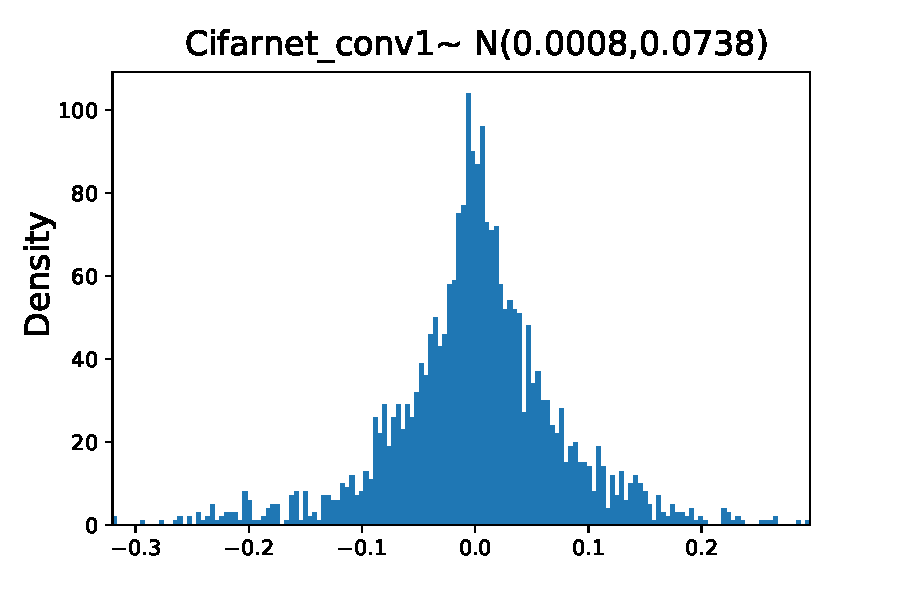
\includegraphics[width=1\textwidth]{ActualWeights/Cifarnet/conv1/Distribution.pdf}
        \end{minipage}
    }
    \subfloat[Resnet-18 conv1]{
        \label{Resnet-18-conv1}
        \begin{minipage}[t]{0.24\textwidth}
        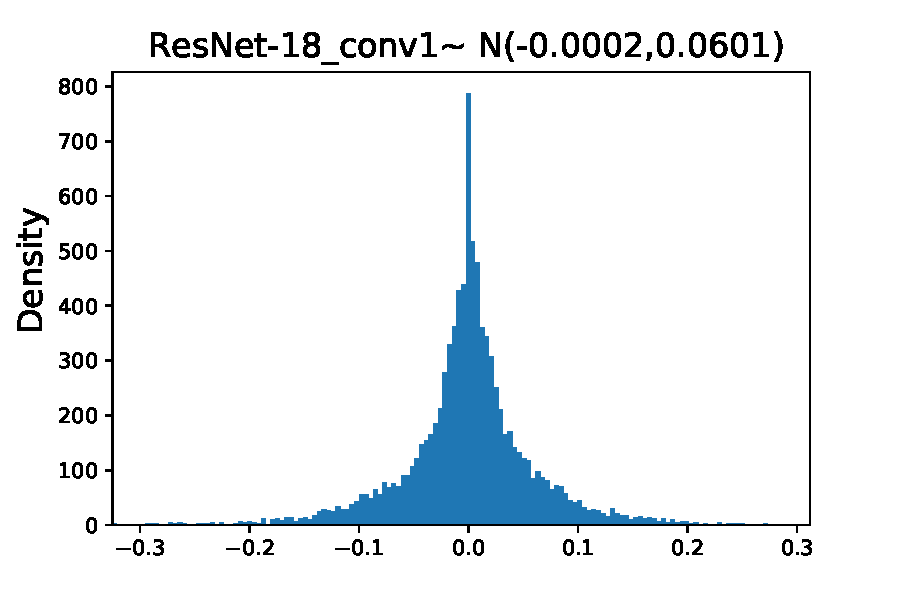
\includegraphics[width=1\textwidth]{ActualWeights/Resnet-18/conv1/Distribution.pdf}
        \end{minipage}
    }
    \caption{The weights of first convolutional layer of cifarnet \citep{krizhevsky2009learning} and Resnet-18 \citep{he2016deep}.}
    %approximately obeying the normal distribution.}
    \label{fig:nd}
    \vspace{-4mm}
\end{figure}

Data quantization is one of the most commonly used methods for network compression~\cite{han2015deep}. 
It aims to reduce the bitwidth of the co-efficient data with the tolerance of a certain loss of the precision for the original data~\citep{zhou2016dorefa,hubara2016binarized,han2015deep}.
% , and achieve a trade-off between the bit width and the data loss.
The low bit width of the representation of data directly reduces the memory footprint of the model, energy consumption and computing requirements~\cite{gysel2016hardware,rastegari2016xnor}.
Consequently, the quantized models can be deployed into resource-limited devices easily~\citep{zhou2016dorefa,ghasemzadeh2018rebnet}.

Current data quantization methods for DNN compression are mostly based on empirical guidance~\cite{} and experimental verification~\cite{}, lack of theoretical analysis and support.
Existing solutions encountered some difficulties: bad trade-off, depending on manual parameter settings and ignoring the distribution of the raw data.
\paragraph{Bad trade-off}: 
The current methods are hard to achieve the trade-off between bit width and data loss\footnote{Data loss refers to the loss of data before and after quantization}. Binary \citep{hubara2016binarized} or Ternary \citep{TWNs} have the fixed low bit width (1/2bit), but a large data loss. The fixed point quantization \citep{gysel2016hardware} can achieve a low data loss, but hard to achieve a low bit width.
\paragraph{Manually setting parameters}: 
Most existing data quantization methods squeeze the data to be quantized within a fixed number of bits by introducing a scaling factor to change the data range. The scaling factor is usually selected based on manual design, by data statistics and experimental verifications of the trained results. 
\paragraph{Ignoring data distribution}: 
Representative works such as Dorefanet \citep{zhou2016dorefa} and Hardware \citep{gysel2016hardware} have quantized the weights to different bit widths and given a well experimental results, but they did not explicitly state the conditions that the input data needs, and hard to guarantee the effectiveness for all situations. 

According to the derivation hypothesis \citep{nasrabadi2007pattern} of the L2 regular term, the weights of the layers in a DNN \textcolor{red}{approximately} follow normal distribution. 
As an instance, Figure~\ref{fig:nd} shows the distribution of the weights of the first layer from two classical models.
%However, existing quantization methods failed to consider this feature and lost the opportunity for analytical quantization during model training.
The ignorance of the distribution of the data in the theoretical analysis brings worse quantization performance.

In order to provide better trade-off between bit width and data loss and quantitatively analysis the loss of the data quantization, in this paper, we propose an ultra-low data loss quantization method called $\mu$L2Q. 

Our method considers the distribution of the data to be quantized, and guarantees 
that any data set that satisfy the distribution hypothesis can achieve the ultra-low data loss with our quantization.
% In addition, our method can achieve ultra-low data loss for any bitwidth quantization.
We summarize our contributions as the following:
%\textcolor{red}{(Cong: the contributions need further polishing; will come back later)}
\begin{itemize}
    \item We propose an effective ultra-low loss quantization  method  ($\mu$L2Q)  which  can  find  the  optimal discrete subspace from the contiguous space, minimizing the loss of data  mapping with our quantitative analysis.
    \item \textcolor{red}{Giving the optimal $\lambda$ set for different  bit  widths, ensuring that the optimal solution can be obtained based on the giving $\lambda$ set over a given bit width}. \textcolor{red}{Yao: The $\lamda$ firstly appears here, so we need to change into a general way or explain it in advance.}
    \item Merging $\mu$L2Q into Caffe framework for training compression and achieve ultra-low inference accuracy loss by taking advantage of our proposed method.
\end{itemize}

The rest of this paper is organized as follows. Section~\ref{sec:backandmo} briefly introduces the existing quantization method in DNN training and presents how the current situation motivates our design. Section~\ref{sec:ulq} presents the proposed precision loss analysis model and our methodology. The optimality analysis and algorithm implementation as well as deployment in model training are presented in Section~\ref{sec:algo}. We compare the trained performance to \sArt ~studies and proved the effectiveness of our solution in Section~\ref{sec:exp}. We conclude this paper in Section~\ref{sec:con}.
\section{Background and Motivation}\label{sec:backandmo}
% Data quantization is a straightforward and effective method for DNN compression to reduce memory access and avoid floating point operations for the deployment of DNNs on hardware~\cite{han2015deep,FPGAAccsurvey}. 
% Our motivation is based on the shortage of the existing quantization methods and focuses on providing a more accurate theoretical support to improve the data quantization loss, hence, improve the trained accuracy of DNN models.
In this section, we first introduce the premise data distribution assumption of DNN designs. Then we conclude the existing data quantization methods. We finally discuss our motivation based on the data distribution assumption and the shortage of the existing solutions.

\subsection{Data distribution analysis}
The assumption of normal data distribution is widely used in DNN related applications.
% Because of the derivation of the L2 regularization term is based on a prior knowledge that the network weights are normally distributed~\citep{nasrabadi2007pattern}.
% Most of the DNN studies explicitly or implicitly assume that the weight or feature data are normally distributed.
For a DNN model, let $X$ be the input features, $y$ be the classification result, and $\omega$ be the weights of the model.
According to the Bayesian posterior probability~\citep{nasrabadi2007pattern,robert2014machine}, the following formula can be obtained:
    \begin{equation}
       p(\omega|X,y) \propto p(X,y|\omega)p(\omega)
    \end{equation}
%\textcolor{red}{(Cong: need explanation. what is function $p()$?)}
%\textcolor{blue}{(Cheng: 
Here $p(\omega|X,y)$ is the maximum posterior probability of deriving $\omega$ from data $\{X,y\}$, $p(X,y|\omega)$ is the likelihood function, and $p(\omega)$ is the prior probability of $\omega$.
Assume $p(\omega_i) = \mathcal{N}(\omega_i|\mu,\sigma^2)$,
the maximum log likelihood of the above formula can be written:

\vspace{-2mm}
\begin{equation}
        l(\omega)=\log(p(X,y|\omega))-\lambda\sum(\omega_i)^2,\,(\mu=0,\sigma=\sqrt{\frac{1}{\lambda}})
    \end{equation}

where $\lambda\sum(\omega_i)^2$ is the L2 regularization term.
These proof that all models based on L2 regular terms training approve the basic premise assumption, which means the weights of the models are normally distributed~\citep{nasrabadi2007pattern,robert2014machine}.
All of the models trained with Caffe framework~\citep{jia2014caffe} are using the L2 regular terms by default~\citep{lecun1998gradient,krizhevsky2009learning,simonyan2014vgg}.
% In batch-normalization \citep{ioffe2015batch} and some data pre-processing algorithms (PCA/ZCA), they also assume the feature data satisfy with the normal distribution.

\subsection{Existing quantization methods}
Existing data quantization methods can be divided into several categories based on the different quantization goals:
1) Binary quantization and 2) Ternary quantization and 3) Fixed-point quantization.
\subsubsection{Binary quantization}
Binary quantization \citep{hubara2016binarized,zhou2016dorefa}, which use a 1 bit binary data to represent the original floating point data.
The classic binary quantization is implemented as \citep{zhou2016dorefa}:
\begin{equation}
    w_q=E(|w_f|)\times sign(w_f)
\end{equation}
Here $E(|w_f|)$ is the mean of absolute value of full precision weights $w_f$ as the scaling factor, and $sign(w_f)=2\mathbb{I}_{w_f\ge 0}-1$, which is either -1 or 1.
Binary quantization is efficient and could achieve up to 32$\times$ compression ratio \citep{hubara2016binarized}. Moreover, binary quantization can completely avoid time-consuming multiplication and convert it into binary operations \citep{rastegari2016xnor}, which dramatically accelerates the computing.

However, current binary quantization methods set scaling factor based on empirical guidance.
The single bit data also cause a high loss for the data representation, easily lead to a high model accuracy loss. 
More importantly, directly binarizing the original DNN model makes is hard to converge during model training and always requires model redesign\citep{ghasemzadeh2018rebnet}.

\subsubsection{Ternary quantization}
Inspired by binary quantization, ternary quantization use three values in 2 bits ($\{-1,0,1\}$) and one or two corresponding scaling factors to represent a set of data \citep{TWNs,zhu2016trained, zhu2016trained,TWNs,alemdar2017ternary,jin2018sparse}. 
Ternary quantization is usually implemented as the following method~\citep{TWNs}:
\begin{align}
    w_q&=
    \begin{cases}
    \alpha&:\,w_f>\Delta\\
    0&:\,|w_f|\le \Delta\\
    -\alpha&:\, w_f<-\Delta
    \end{cases}\\
\alpha &=\underset{i\in\{i| |w_f(i)|>\Delta\}}{E}(|w_f(i)|)
    ~\&~ \Delta = 0.7E(|w_f|) \nonumber
\end{align}
where $\alpha$ is the scaling factor and $\Delta$ is the threshold for quantization. 
%\begin{align}
%    \Delta &= 0.7E(|w_f|)\nonumber\\
%    \alpha &=\underset{i\in\{i| |w_f(i)|>\Delta\}}{E}(|w_f(i)|)
%\end{align}

Moreover, the method proposed in \citep{TWNs} solve the optimization problem of minimizing L2 distance between $w_f$ and $w_q$, which implicitly includes the assumptions that the distribution of $w_f$ satisfies normal distribution.
Since ternary uses 2 bits for data representation, its data loss and accuracy degradation is smaller than binary quantization but remains high.
% Besides, ternary usually uses 2 bits to represent three values, and the bit width resources are not fully utilized.
\subsubsection{Fixed-point quantization}
\label{sec:fixed-point}
Fixed-point quantization is the most commonly used quantization method due to it is simplicity~\citep{zhou2016dorefa,gysel2016hardware,lin2016fixed}.
% , which is achieved by moving the decimal point by shifting operation on a hardware.
There are various implementations for fixed-point quantization~\citep{gysel2016hardware, zhou2016dorefa}. 
Overall, it reserves the integer and fractional part of a floating point data within a limited bit width.
% The work in \citep{gysel2016hardware} reserves the integer and fractional part within a limited bit width to adapt to the representation of the hardware, and adjusts the decimal point position $p$ by setting the length of the two parts.
% The work \citep{zhou2016dorefa} first shifts the decimal point by $p$ bits, then preserves the integer part in front of the point and discards the decimal part after the point.
For the floating array data $w_f$ to be quantized to $w_q$ with $k$-bit width,
the implementation for fixed-point quantization is as follows:
 \begin{equation}
 \label{fixed-point-quantization}
     \begin{cases}
         p=\lfloor \log_2(max(|w_f|)) \rfloor-(k-2)\\
         w_q=Round(\frac{w_f}{2^p})
     \end{cases}
 \end{equation}

Here $p$ is the steps that need to be shifted, which is calculated based on the limited $k$-bit width,  to ensure that the quantized data does not overflow within $k$-bit width. $w_f$ is an array, and $max()$ is the function for computing the maximum value of the array. Fixed-point quantization will give priority to the value in high bit, so our reserved bits will start with the highest bit of the absolute maximum value of the array, and we calculate p according to this logic. Here is $(k-2)$ instead of $(k-1)$ since the sign bit is taken into consideration.

Fixed-point quantization always gives priority to retain the data with larger absolute value and losing the data with smaller absolute value.
% Its loss function can be expressed as:
% \begin{equation}
    % \label{eqn:loss_of_fixed}
    % J=\lVert w_q-w_f\rVert_2^M
% \end{equation}
% Here $M$ is a great integer and represents for paying much attentions to the high bits loss and less for low bits. But it do not work when quantizing to low bit widths in most models. Based on our analysis, the weights or activations of many current models are approximately obeying a normal distribution. On one hand, the loss function does not conform to the normal distribution of most models' weights or activations. On the other hand, in the normal distribution, the great value part only occupies a small proportion. When the quantized bit width is low, the strategy of retaining the high bits will cause most of the valid values, nearing the mean, to be discarded, resulting in great data loss. $w_q$ and $w_f$ are the value after quantization and the full precision value. 
%\textcolor{red}{(Cong: also, a little explanation would be nice here. What does this $\lVert xx \lVert_2^ \infty $ mean?)}
%\textcolor{blue}{(Cheng: 
%Here $M$ is a great integer and this formula can be explained from two aspects as follows: Firstly, $J$ pay all attention to the large bias, that is, the discarding of high bit values will cause the much more quantization loss than the discarding of low bit values. Secondly, from the perspective of discrete point fitting \citep{nasrabadi2007pattern} in machine learning, this formula always focuses on the outliers, ie discarding the high bit will create a distinct outlier, rather than the overall distribution of the sample. From this perspective, fixed-point quantization is not good at fitting.)}

% The fixed-point quantization ignores the fact that data $w_f$ follow the normal distribution in \eqnref{eqn:loss_of_fixed}. In addition, when $k$ is small ($k<8$), the loss of fixed-point quantization will be large since it discards most of the valid data. In general, fixed-point is hard to be applied in an ultra-low bit width quantization in practice.

\subsection{Motivation}
%1、问题:权值量化过程中的数据损失和位宽的权衡
% Data quantification is a commonly used method of network compression. It tried to produce a model with a low bit width whose output is similar to the full precision one's output. 
% The low bit width directly affects some aspects of the DNN model, such as low memory footprint, low energy consumption, and high computing speed, but often also leads to degradation in accuracy. The challenge is to achieve a trade-off between data loss and bitwidth.
%2、当前一些方法的weakness:
% The current methods have some difficulties in achieving the trade-offs. 
%   binary/ternary数据损失过大,而且在分析和改进方面存在一些困难
%The binary/ternary \citep{hubara2016binarized,TWNs} quantization has large accuracy degradation and are inflexible, which is hard to trade off between accuracy and bit width.
The previous quantization methods are good, however, they are either require manually designed parameters or based on emperical and experimental guidance and are lack of theoretical analysis, which are hard to achieve good trade-offs. 
For example, The Bianry \citep{hubara2016binarized} / Ternary \citep{TWNs} are classic works, but they has large accuracy degradation and are hard to quantitatively control the trade off between accuracy and bit width.
The Fixed-point quantization \citep{gysel2016hardware,zhou2016dorefa} are difficult to achieve a trade-off between data loss and bit width because of its poor performance at low bit widths.

The issues above motivate us to take the \textbf{data distribution} into consideration, evaluate our data loss by establishing a credible data \textbf{loss function}, then find an optimal solution to achieve the lowest loss for the \textbf{quantization}.
A solution that solves the optimal data quantization at all different bit widths to achieve a trade-off between bit width and data loss is proposed, named $\mu$L2Q.
% In our experimental part, we demonstrate that $\mu$L2Q achieves better trade-offs between bit width and data loss compared to the state-of-the-art methods in normal distribution data, and also achieves better trade off between model accuracy and weight bitwidth in model training. 
%need to say
%\textcolor{red}{(Cong: this section for motivation is too verbose (LOL sorry for being mean). Need to greatly delete some paragraphs. Also it is not well organized... really need to work again on this section. I feel we just need to explain several points: 1) previous works do not consider data distribution; 2) previous works do not consider quantitative analysis for quantization loss, so they cannot control how much the precision loss is, i.e., trade-off between performance and accuracy. Will come back later for this section.}
%\textcolor{blue}{(Cheng: sorry for this, I just remove the redundancy.)}

%We realize that making assumptions about raw data is critical. First, it limits the problem to a certain scope, rather than trying to solve all problems in one way. Second, it makes our approach analyzable, and we can try to solve problems using math or machine learning tools. The quantization loss is a more direct metrics than the output accuracy of the model, which directly shows the difference between the data before and after the quantization. Based on the assumption of data distribution, we derive the analyzable  quantization loss function. The flexibility of quantification is the key to achieving accuracy and bit width trade-offs. Based on analyzable quantization loss function, we design the method that the quantization loss is guaranteed to be optimal in all bit widths, and realize the flexible quantization. 

%Most of the previous works on quantification was based on empirical guidance or experimental verification. In addition, binary and ternary are concentrated on ultra-low bit width quantization, but there is a large quantization loss compared with the original data. Meanwhile, the fixed-point quantization can only be applied to multi-bits quantization. For example, between these bit widths, the 4-bit width is not available for fixed-point quantization (the loss of fixed-point quantization with 4-bit width is large). Our approach is based on a theoretical analysis of the assumption and maintains low loss over all bit widths.

%Quantization is a hot issue of network compression, which can reduce the size of model storage, while at the same time designing for fast and low-power computing. 

%1、各种量化方法难以直接比较,基于模型输出的比较不可信(在该论文中表示量化输出甚至比全精度的高)
%The current quantization methods are often based on empirical guidance, but lack of assumptions and theoretical analysis. Moreover, it is difficult to directly compare existing quantization methods.  Firstly, the various quantization methods focus on different points, some focus on speed, while others focus on the trade-off between accuracy loss and compression ratio. Secondly, since the complexity of the deep models, there are too many reasons for its accuracy. For deep networks of the same structure, using different hyper-parameters will give completely different results. Even if the same external condition is used, the results of two training process may be different. Therefore, there is no convincing based on the comparison of model accuracy. Especially for large deep networks with redundancy, it is difficult to come up with convincing results, because the gaps of different methods are often small, and even some models have higher accuracy after compression than the full precision model \citep{zhu2016trained}.

%2、没有一种可以适应不同位宽的量化方法,以不同深度(冗余)的网络的量化
%Moreover, the existing quantization methods do not propose functions that smoothly adapt to different network models. Binary and ternary quantization focus on high compression ratio and speed, but with large loss. The fixed-point quantization is very simple and fast, based on which some tradeoffs between precision loss and compression ratio can be achieved, but it is difficult to achieve high compression ratio. Experiments show that under our assumptions, the loss of fixed-point quantization with 4 bit width has been larger than the loss of ternary quantification (only 2 bit).

%3、存在一些补救措施,但是治标不治本(这两篇文章都是残差二值化相关的)
%There are also some remedies. For example, the residual binary quantization \citep{ghasemzadeh2018rebnet,li2017performance} is used to reduce loss of binary quantization, but its essence is to superimpose multiple binary quantization processes to reduce the loss, while increasing complexity and reducing the compression ratio.

%4、我们所做的一些工作
% In this paper, firstly, we make a reasonable assumption about the premise of network compression. Secondly, inspired by the previous works, we proposed our quantization method called $\mu$L2Q, which can flexibly adapt to various network models with different bit width. Thirdly, based on our initial assumption, we give the data loss function, which be used in our experiments as the direct evaluation measure.
%fully analyzing the ULQ parameter selection and gave an approximate optimal solution. Finally, it is verified by experiments that ULQ can achieve the lowest loss in all bit widths compared to the current quantization methods, that is, the optimal trade-off of precision loss and bit width can be found.
%做环境假设,即正态分布的假设
\section{Proposed Method}\label{sec:ulq}

In order to quantize the weights with an ultra-low loss, we design the $\mu$L2Q method based on the assumption of normal distribution for the input data. 
We use a loss function to evaluate our proposed $\mu$L2Q method, are The low loss training quantization is achieved by illustrating the low loss data quantization for the co-efficients during the model training. 

\subsection{Loss function design}
The quantized data is represented as $w_q$, and the process of quantization can be simply expressed as follows:
\begin{equation}
    w_q=Quantize(w_f)
\end{equation}

The $Quantize()$ is a quantization function, which maps $w_f$ to $w_q$, where $w_q$ are generally represented with integer. 
Based on the discussion in Section~\ref{sec:backandmo}, $w_f$ obeys normal distribution, so the quantized loss function of it could be simplified as follows:

\vspace{-2mm}
\begin{equation}
\label{eqn:loss_func}
    J=\lVert w_f-w_q \rVert_2^2
\end{equation}

where $J$ is the distance between $w_f$ and $w_q$, which is to be minimized.
%\textcolor{red}{(Cong: here $w_f$ and $w_q$ refers to all input/output data, right? Or just one weight? If it is for a large bunch of data, I feel the computation of $J$ needs to be better defined. For example given 1M weights, how to compute $J$ over 1M data? Is it summed up or averaged?)}
%\textcolor{blue}{(Cheng: $w_f$ is an array, it can be the weights of one layer in the network models, or the activations or outputs of one layer. Here, we abstract them into an array $w_f$ that satisfies a normal distribution.)}
Considering the complexity and uncertainty based on the output of DNN models, instead of measuring the final DNN output accuracy, we use $J$ as the direct evaluation metric to evaluate the quantization loss.

\subsection{Ultra Low Loss Quantization ($\mu$L2Q)}

$w_q$ always has a loss to represent $w_f$ in a limited bit width.
Binary and ternary quantization methods use additional scaling factor to reduce the quantization loss. The position parameter (i.e. $2^k$) for fixed-point quantization can also be regarded as a scaling factor~\cite{zhou2016dorefa,gysel2016hardware}. 
%It can be concluded that the scaling factor is an effective way to reduce the quantization loss.
%We follow the same design strategy in our method.

Given data $w_f$ which follow the normal distribution as $w_f\sim \mathcal{N}(\mu,\sigma^2)$, the process of transforming it into a standard normal distribution is as follows:
\begin{equation}
    \label{eqn:snd}
    \varphi=\frac{w_f-\mu}{\sigma}\sim \mathcal{N}(0,1)
\end{equation}

Inspired by the scaling factor and transforming of normal distribution, we set our scaling factor $\alpha$ and offset factor $\beta$ as follows:
\begin{equation}
    \begin{cases}
    \alpha=\lambda \sigma\\
    \beta=\mu
    \end{cases}
\end{equation}
where $\lambda$ is adjustable parameter that scales the data to the range we need to quantize, where:
\begin{equation}
\label{eqn:distribution_scale}
 \frac{w_f-\beta}{\alpha}=\frac{\varphi}{\lambda}\sim \mathcal{N}(0,\frac{1}{\lambda}).   
\end{equation}

The scaling factor and shifting factor are used to transform the general normal distribution to the standard normal distribution, and then scaling it to the integer range that we could quantize with a given bit width. Binary/ternary has an manually designed scaling factor that is used to scale the binary/ternary value range to reduce quantization loss. For fixed-point quantization, we find the fact that the shift steps can be regard as its scaling factor. It can only be an form of $2^n$ ($n$ is an integer).

In addition, $\lambda$ is the segmentation width. 
Let the bit width be $k$-bit, so the distribution $\varphi$ in \eqnref{eqn:snd} will be cut into $(2^k+1)$ segments by the quantization location with the interval of segmentation width $\lambda$.
The data in the $(2^k+1)$ segmentations will be quantized to $2^k$ numbers by the principle of proximity or nearest neighbors (from \figref{fig:before_ulq} to \figref{fig:after_ulq}).
%\textcolor{red}{(Cong: in Fig. 2, what is the value of $k$ and $\lambda$? Needs to explain.)}


%To be general, we propose a full-precision scaling factor $\alpha$ and an offset factor $\beta$ that can quantize any data in normal distribution into integer values. The scaling factor can reduce the quantization loss, while the offset factor can eliminate the impact of the mean shift of the distribution.

%\textcolor{red}{(Cong: Sorry I have a personal question. What is the difference between the scaling factor in Binary/Ternary and the scaling factor in fixed-point quantization? Why the fixed-point scaling factor is a low-precision factor?)}
%\textcolor{blue}{(Cheng: Our approach is essentially based on the analysis of standard normal distributions. )}
Comparing with the customized or low-precision scaling factors in binary/ternary and fixed-point quantization, $\mu$L2Q only requires one simple scaling factor and offset factor representations that is directly related to the data loss. 
%Fortunately, we noticed the calculation from the general normal distribution to the standard normal distribution, including the parameters we needed.


%\begin{figure}
%    \centering
%    \includegraphics[width=0.8\columnwidth]{fig/out.pdf}
%    \caption{The quantization locations in a normal %distribution.
%    Interval of any two nearest locations is $\lambda$. All %data of distribution will be quantized to several numbers ($2^k$) located in quantization locations.
%    \textcolor{red}{Plot two figures instead of one.}}
%    \label{fig:segmentation}
%\end{figure}

$\mu$L2Q can be concluded as the following equation:

\begin{equation}
    \label{eqn:ulq_method}
    w_q = Round(\underset{(1-2^{k-1},2^{k-1})}{Clip}(\frac{w_f-\beta}{\alpha} + 0.5))
\end{equation}

Here $Clip$ is a function to enforce the values outside of the representation range being replaced by their nearest neighbors ($(1-2^{k-1})$ or $(2^{k-1})$).
%Generally, the minimum and maximum values will always exceed the range that the k-bit width can represent, that is, outside the range of $[1-2^{k-1}, 2^{k-1}]$.
The offset of 0.5 is to shift the mean of the distribution, which shifts the scaled quantization locations (scaled by $\frac{1}{\lambda}$) to integers. It constrains the quantized value to start from the mean of the distribution as well as reducing the quantization loss.
%and ensures that an even count of quantized values are taken, since for any given $k$-bit width, there always have $2^k$ values can be represented, and the values count is even.
%\textcolor{red}{(Cong: why does 0.5 can ensure the number of vaules is even? why need it to be even? Sorry for being stupid...)}
%\textcolor{blue}{(Cheng: When the data is scaled (by $\frac{1}{\lambda}$), the quantized position nearest to 0 is exactly -0.5 and 0.5, so we make a 0.5 offset just to move the quantized position to the integer. If no shift is done, the quantized value will start from the mean of the distribution, and the quantization loss is not minimal.)}



\begin{figure}[hbp]
    \centering
    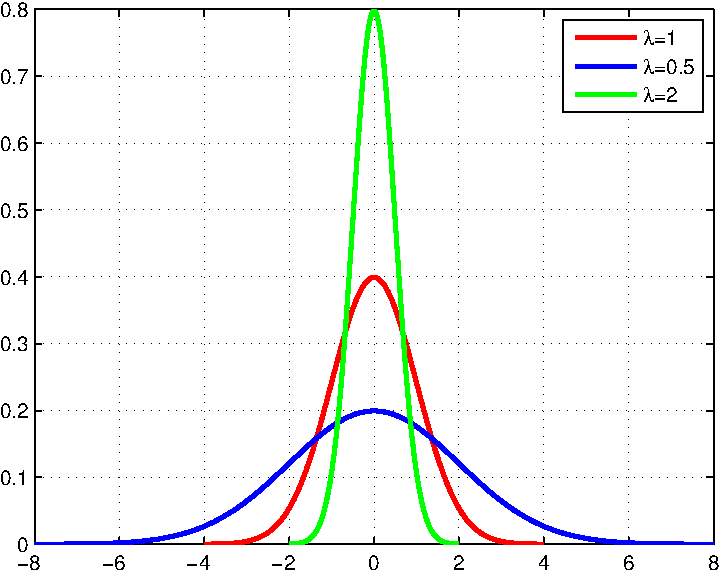
\includegraphics[width=0.6\columnwidth]{Simulation/different_lambda.pdf}
    \caption{$\lambda$ can scale the standard normal distribution to the different range according to the \eqnref{eqn:distribution_scale}.}
    \label{fig:differentlambda}
    \vspace{-2mm}
\end{figure}
\begin{figure*}[!htp]
    \centering
    \subfloat[Raw Data Distribution]{
        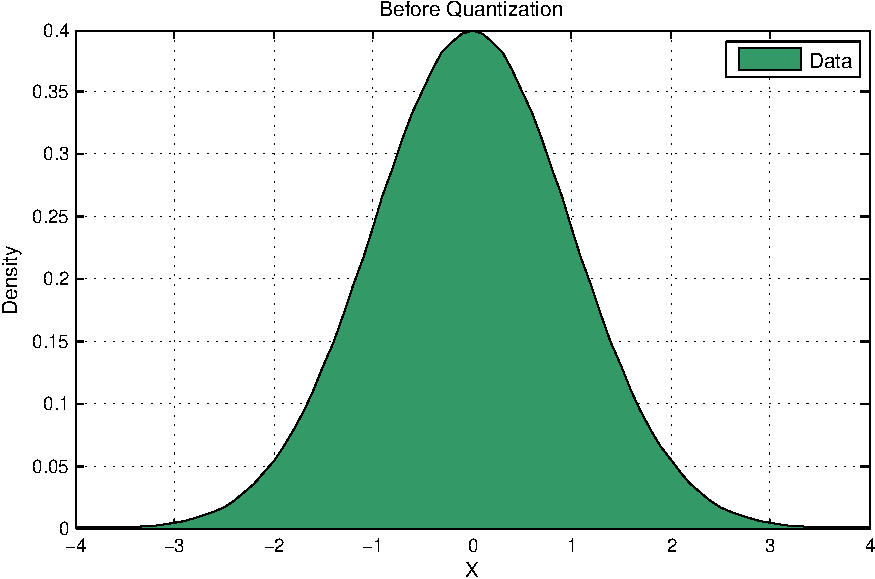
\includegraphics[width=0.33\textwidth]{fig/raw_distribution_croped.pdf}
        \label{fig:before_ulq}
    }~~~~~~~~~~~~~~~~
    \subfloat[Split Data to Regions (R)]{
        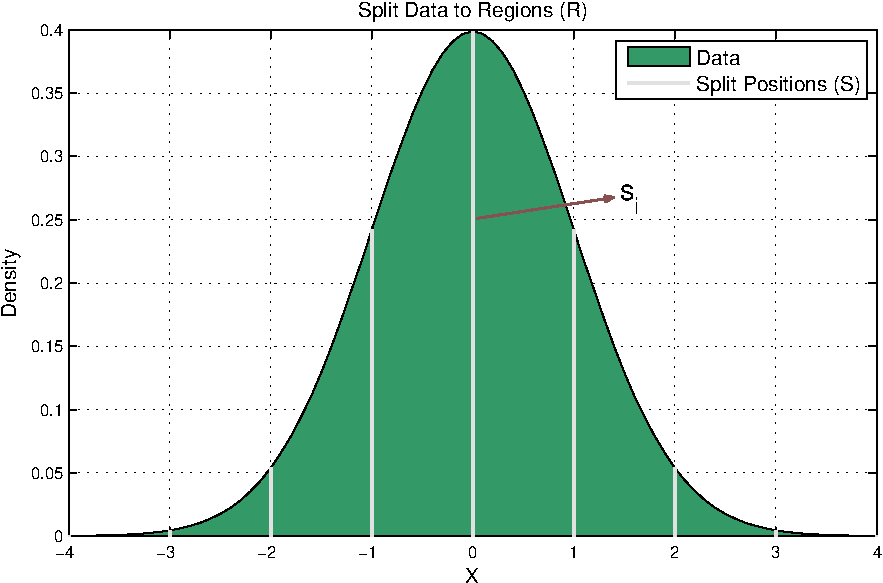
\includegraphics[width=0.33\textwidth]{fig/SplitData2Regions_croped.pdf}
        \label{fig:split_data}
    }\\
    \subfloat[Finding the optimal quantization $q_i\in Q$]{
        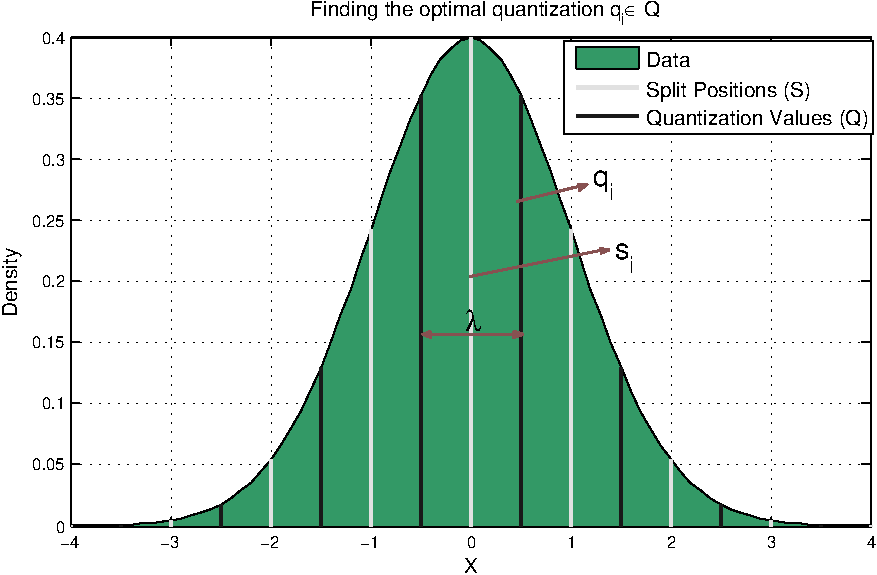
\includegraphics[width=0.33\textwidth]{fig/FindingOptimalQuantization_croped.pdf}
        \label{fig:find_q}
    }~~~~~~~~~~~~~~~~
    \subfloat[Using $q_i$ to represents data in $R_i$]{
        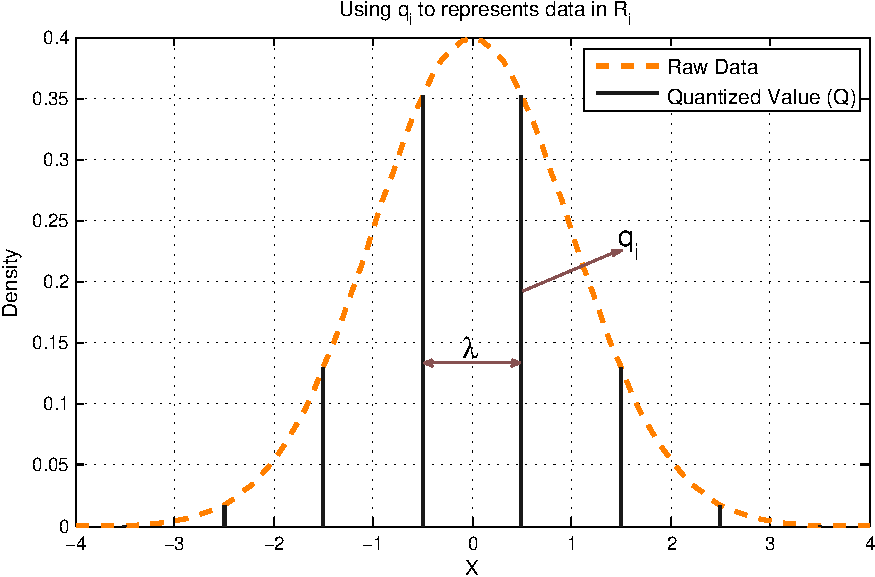
\includegraphics[width=0.33\textwidth]{fig/Q2RepR_croped.pdf}
        \label{fig:after_ulq}
    }
    \caption{The quantization process of $\mu$L2Q. $\varphi$ is the raw data in \figref{fig:before_ulq}, and it be split to $n$ regions $R_i$ by split positions S as shown in \figref{fig:split_data}. The next step is to find the optimal quantization value $q_i\in R_i$ which shown in \figref{fig:find_q}. Finally, all the data in $R_i$ are represented by $q_i$ as shown in \figref{fig:after_ulq}, and our quantization process is done.}
    \label{fig:ulq_process}
\end{figure*}
\section{Optimal Implementation}\label{sec:algo}
%理论到实现需要解决的一些问题
%1、最优位置不等宽
%2、实际中一些位置是没有数据的
%最优量化位置分析:在什么地方量化,损失是最小的
%Based on the discussion above, 
The value of $\lambda$ which is discussed above is the critical factor for low data quantization loss. 
It is used to scale the standard normal distribution to the appropriate range to ensure the lowest data loss after quantization. For example, as shown in \figref{fig:differentlambda}, the data can only be quantized to 4 integers when $\lambda=2$, but if $k>2$, the extra bit width cannot hit the valid data, it caused a waste of bitwidth resource.
When $\lambda=0.5$, data can be quantized to 16 integers, but $k < 4$, the entire data distribution cannot be effectively represented.
So a globally optimal $\lambda$ needs to be analyzed and achieved to solve the issue.

\subsection{Optimality analysis}
To simplify the issue of finding the optimal $\lambda_k$ for $k$-bit width ($k\ge1$), we assume that the quantization is $k$-bit width and let $n = 2^k$.
For the standard normal distribution $\varphi \sim \mathcal{N}(0,1)$, The quantization has three steps:
\begin{itemize}
    \item According to split positions $S=\{s_i|i=1,\cdots,n-1\}$, dividing $\varphi$ into $n$ regions $R_i$.
%\textcolor{blue}{(Cheng: the arrays or sets of value in different range within $\varphi$, that is, $R_i$ is the subset of $\varphi$: $R_i \subset \varphi$.)} 
\begin{equation}
    R_i = \begin{cases}
    \{\varphi_j|\varphi_j>s_{n-1}\};& i=n\\
    \{\varphi_j|s_{i-1}<\varphi_j\le s_{i}\};& i=2, \cdots, n-1\\\
    \{\varphi_j|\varphi_j \le s_1\};&i=1\
    \end{cases}
\end{equation}
%\textcolor{red}{(Cong: what is split position $s_i$? Are they floating point fractional values?)}
Here, $s_i$ is the floating value, and based on $s_i$ the raw data are split to two parts $\{R_i,R_{i+1}\}$ and $R_i \subset \varphi$.
\item  Finding the optimal quantization value $q_i$ in $R_i$; %\textcolor{red}{(Cong: $q_i$ are fixed point values?)}
%\textcolor{blue}{(Cheng: On this section, $q_i$ is floating value, and all the data within $R_i$ will be quantized to $q_i$, that is, all the data in $R_i$ has the same value $q_i$. The optimal meaning is that the loss before and after quantization is minimal.)}
\item Using $q_i$ to represent all values in $R_i$. 
\end{itemize}
Finally, all data in $\varphi$ are quantized into $n$ values, denoted as $Q=\{q_i|i=1,\cdots,n\}$. 
Easy to know, $\lambda=|q_{2}-q_1|=\cdots=|q_{i+1}-q_i|=\cdots=|q_{n}-q_{n-1}|$. Detailed steps are shown in \figref{fig:ulq_process}.%$\lambda$ should be any $|q_{i+1}-q_i|$ but not $|s_{i+1}-s_{i}|$.
%\textcolor{red}{(Cong: what does it mean by "lamda should be any $|q_{i+1}-q_i|$"? Does it mean the value of $\lambda$ equals to any $|q_{i+1}-q_i|$?)}
%\textcolor{blue}{(Cheng: that is $\lambda=|q_{2}-q_1|=\cdots=|q_{i+1}-q_i|=\cdots=|q_{n}-q_{n-1}|$.)}

We define the optimization goal as:
\begin{equation}
    S^*,Q^*=\underset{S,Q}{\arg\min}(J)
\end{equation}
%\textcolor{red}{(Cong: $S*$ and $Q*$ should be defined first or explained here.)}
$S*$ and $Q*$ are the optimal $S$ and $Q$ which make the quantization loss $J$ minimal. $J$ is the loss function defined in \eqnref{eqn:loss_func}.
It could be further expressed with $R_i$ and $q_i$, $J$ as follows:
\begin{align}
\label{eqn:analysis_loss}
        J&=\lVert \varphi-Q \rVert_2^2\nonumber\\
        &=\sum_{i=1}^n(|R_i|q_i^2)-2\sum_{i=1}^n(q_i\sum R_i)+\lVert\varphi\rVert_2^2
\end{align}
Here, $\lVert\varphi\rVert_2^2$ is a constant value that is independent from $Q$ and $S$, and $|R_i|$ denotes the number of elements in $R_i$.
%\textcolor{red}{(Cong: this equation needs to be explained. The $R_i$ are the "regions" defined above; how can a "region" being used in a equation? Does $R_i$ has a value?)}
%\textcolor{blue}{(Cheng: $R_i$ is an array and $R_i \subset \varphi$.)}
We can derive the optimal value of Q as follows:
\begin{align}
    \frac{\partial J}{\partial{q_i}}&=2|R_i|q_i-2\sum{R_i}=0\nonumber\\
    &\Longrightarrow q_i^*=\frac{\sum{R_i}}{|R_i|}=\mu_i
\end{align}

It means, when $q_i^*$ equals to the mean $\mu_i$ of $R_i$, the loss $J$ can be minimized. Based on this, we substitute $q_i^*$ into \eqnref{eqn:analysis_loss} and have:
\begin{equation}
\label{eqn:analysis_C}
    S^*=\underset{S}{\arg\max}(\sum_{1}^{n}(|R_i|u_i^2))
\end{equation}
\eqnref{eqn:analysis_C} has no straightforward solutions. Fortunately, our problem premise is $\varphi\sim \mathcal{N}(0,1)$, so we can approximate this problem by enumerating.
%\textcolor{red}{(Cong: what does "exhausting discrete values"? Do you mean enumerating?)}
%\textcolor{blue}{(Cheng: Yes, it means enumerating.)}

\subsection{Optimal Solution}
Since $\varphi$ in \eqnref{eqn:snd} is known, and it is a standard normal distributed data, we can list all possible situations and find the optimal solution. Our method only finds one parameter $\lambda$, i.e., all $|q_{i+1}-q_{i}|$ should be the same $\lambda$. For $\varphi\sim \mathcal{N}(0,1)$ we need to find the $\lambda_k$ for $k$-bit width quantization that minimizes $J$ in \eqnref{eqn:analysis_loss}. 

\textbf{Data:} Specifically, we generate $N=100000$ data set $\varphi$ that follows the standard normal distribution, and list all possible $\lambda_k$ by a certain interval precision, and select the $\lambda_k$ which minimizes $J$ at $k$-bit width.

\textbf{Range:} Easy to know, $\lambda>0$.
For the upper bound of $\lambda$, given $k$ bits, the range of $\lambda_k$ is $(0, \lambda_{k-1}]$ ($k>1$).
%\textcolor{red}{(Cong: why is $\lambda$'s upper bound is $\lambda_{k-1}$?)}
%\textcolor{blue}{(Cheng: From section III we get that the $\lambda$ is the segmentation width for the standard normal distribution. For every increment of k, double segmentations need to be splited within the standard normal distribution. So  the segmentation width will be reduced, that is, the value of the $\lambda_{k+1}\le\lambda_k$, in order to allow the new segmentations to fall in the valid data area.)}
In addition, we can get that, when $k=1$, the optimal quantization location are the means ($\pm\mu_1,\mu_1>0$) of the two sub-distributions which separated from $\varphi$ by $\varphi$'s mean $\mu$, i.e. $\lambda_1=2\mu_1$.
%\textcolor{red}{(Cong: sorry I did not get this.. sorry for being stupid again but this is not easy to get!..)}
%\textcolor{blue}{(Cheng: The case that $k = 1$ is a special case, in which we only need to split the distribution into two segmentations according to one value. Experiments show that when k=1, it is optimal to split the distribution into two segmentations according to the mean $\mu$ of the data distribution.)}

\textbf{Interval precision:} We take $I=1000$ floating point data within the range of $\lambda_k$, that is $(0, \lambda_{k-1}]$ ($k>1$), to ensure the precision of the approximation. The approximate optimal result is shown in \tabref{tab:optimal_lambda}.

We only give $k = 1$ to $8$ results in \tabref{tab:optimal_lambda}, and more results are not much practical. Because after the bit width is sufficient, the results of evenly quantization is good enough.

\renewcommand{\arraystretch}{1.3}
\begin{table*}[htbp]
\center
    \caption{The list of optimal solution $\lambda$, \textbf{Loss} is the minimum data loss calculating by $J$, and \textbf{Precision} is the interval precision for getting $\lambda$.}
    \label{tab:optimal_lambda}
\begin{tabular}{c|c|c|c|c|c|c|c|c}
\hline
k (bit width)                      & 1      & 2      & 3      & 4      & 5      & 6      & 7      & 8      \\ \hline
$\lambda$ & 1.5959 & 0.9894 & 0.5838 & 0.3327 & 0.1897 & 0.1043 & 0.0563 & 0.0304 \\ \hline
\textbf{Loss}                   & 0.3625 & 0.1189 & 0.0374 & 0.0115 & 0.0035 & 0.0010 & 0.0003 & 0.0001 \\ \hline
\textbf{Precision} & 0.0080 & 0.0050 & 0.0029 & 0.0017 & 0.0009 & 0.0005 & 0.0003 & 0.0002 \\ \hline
\end{tabular}
\end{table*}
%
%解决的思路
\subsection{Algorithm implementation}
%完整的实现算法
Although above analysis was based on a special case of standard normal distribution $\varphi \sim \mathcal{N}(0,1)$, this would make the results look less reliable and may be difficult to apply to the different distributions that actually exist. 
However, it should be noted that, as described in \eqnref{eqn:ulq_method}, our method is based on the premise of normalization of any normal distribution data to the standard normal distribution. 

ULQ can be divided into two steps in Logically: 1) normalize the  $w_f$ which satisfies normal distribution to the standard normal distribution, in this step we record the offset factor $\beta=\mu$ and a part of the scaling factor $\sigma$; 2) Based on the standard normal distribution generated in step 1, we then analyze the optimal parameter $\lambda$ selection and get the complete scaling factor $\alpha=\lambda\sigma$.

The above analysis is reasonable and credible, because the second logical step is based on the standard normal distribution. In terms of implementation, we only use one step to achieve the above two steps. $\mu$L2Q as shown in \algorithmref{alg:ulq}.
\renewcommand{\arraystretch}{1.3}
\begin{algorithm}[htbp] %算法开始 
\caption{Ultra-low loss quantization} %算法的题目 
\label{alg:ulq} %算法的标签 
\begin{algorithmic}[1] %此处的[1]控制一下算法中的每句前面都有标号 
\Require  $w_f \sim \mathcal{N}(\mu,\sigma)$, $k\ge 1$ 
\Ensure $w_q$, $\alpha$, $\beta$ 
% if-then-else 
\If{$k>8$} 
\State $\lambda_k=\frac{max(w_f)-min(w_f)}{2^k-1}$ 
\Else 
\State Get $\lambda_k$ from \tabref{tab:optimal_lambda}
\EndIf 
\State $\alpha = \lambda_k\sigma$ \& $\beta=\mu$ 
\State $\varphi = \frac{w_f-\beta}{\alpha}$
\State $clip_{max}=2^{k-1}$ \& $clip_{min}=1-2^{k-1}$
\State $\varphi= Clip_{(clip_{min},clip_{max})}(\varphi+0.5)$
\State $w_q=Round(\varphi)$
\end{algorithmic} 
\end{algorithm}

\subsection{Integration with DNN training}
For each layer $l$ of forward-propagation, we first quantize $w_f(l)$ to $w_q(l)$. 
And then, $w_q(l)$ is used to calculate the output of each layer $l$ in forward propagation.

During back-propagation, the values in \algorithmref{alg:ulq} are not differentiated, derivatives of $w_q$ are computed instead \citep{zhou2016dorefa,TWNs,gysel2016hardware}, yielding the identity function \eqnref{eqn:gradient}, and $g(l)$ is the gradient of layer $l$.
\begin{equation}
    \label{eqn:gradient}
    g(l)=\frac{\partial J(w_q)}{\partial w_q(l)}=\frac{\partial J(w_q)}{\partial w_f(l)}
\end{equation}

%For a deployment of the NN model on any devices for inference, we only need to save the ternary-valued co-efficients and the scaling values together with the other quantized network parameters if necessary.

\begin{figure*}[!ht]
    \centering
     \subfloat[Loss with different bitwidth]{
        \label{fig:Loss_with_bits}
        \begin{minipage}[t]{0.3\textwidth}
            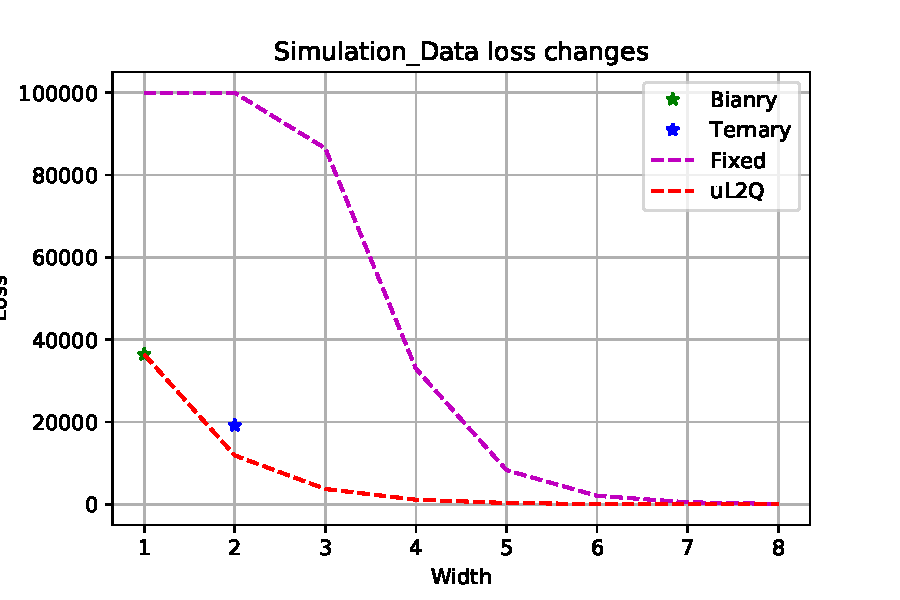
\includegraphics[width=1\textwidth]{Simulation/Bitwidths/LossWithWidth.pdf}
        \end{minipage}
     }
     \subfloat[Loss with different means]{
        \label{loss_with_means}
        \begin{minipage}[t]{0.3\textwidth}
        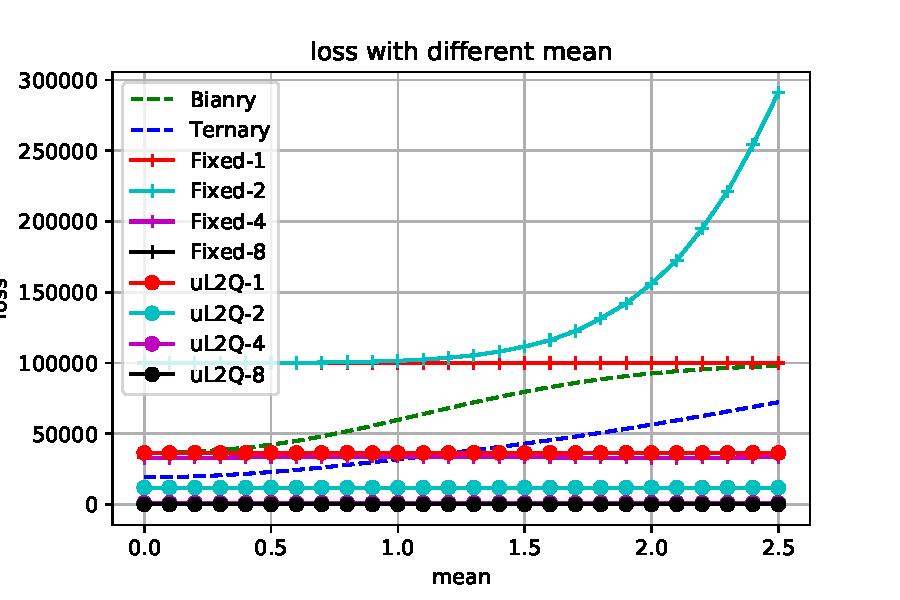
\includegraphics[width=1\textwidth]{Simulation/ShiftScale/loss_with_mean_in_small_range.pdf}
        \end{minipage}
     }
     \subfloat[Loss with different standard deviations]{
        \label{loss_with_sds}
        \begin{minipage}[t]{0.3\textwidth}
        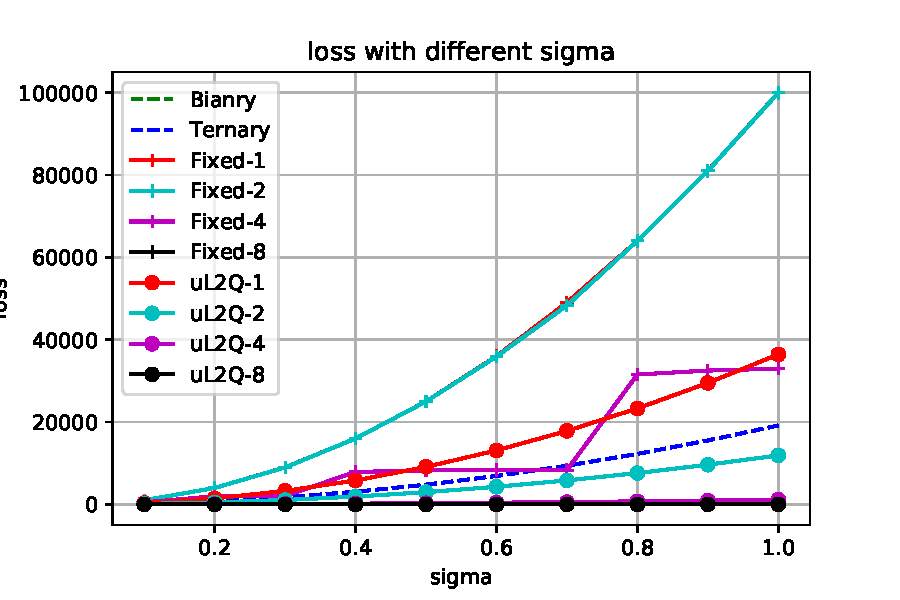
\includegraphics[width=1\textwidth]{Simulation/ShiftScale/loss_with_sigma_in_small_range.pdf}
        \end{minipage}
     }
    \caption{Losses for different means and standard deviations.}
    %distributions. The result of the fixed-point quantization at 8-bit width coincides with the 4-bit and 8-bit width results of our method. Our method is insensitive to mean change and is the most stable for standard deviation changes.}
    \label{fig:loss_with_distribution}
\end{figure*}
\section{Evaluations}\label{sec:exp}
We use both simulated data and DNN model training to evaluate our proposed $\mu$L2Q method.
%The experimental part are divided into three experimental parts: \textbf{simulated distribution analysis}, \textbf{DNN weights analysis} and \textbf{DNN training}. 
\textbf{Simulated data} is used to evaluate the data loss of different quantization algorithms from existing works as well as our proposed solution. 
%Since the generation of analog data is relatively easy, this part of the experiment can comprehensively analyze the comparison results of different quantization algorithms under all different distribution cases.
In the \textbf{DNN model} based evaluations, we first analyze our quantization on some selected model weights trained without our quantization to show the effectiveness of our method. We then illustrate our quantization method as a solution in the current Caffe \citep{jia2014caffe} framework and enabled it for model training and use the final trained accuracy of the models to demonstrate the impact of our $\mu$L2Q method for data quantization. The version of Caffe framework is 1.0.0.

\subsection{$\mu$L2Q on Simulated Data}
\subsubsection{Experimental settings}
We randomly generate $N=100000$ data with normal distribution $\mathcal N(\mu, \sigma^2)$
and consider the impact of 
(1) targeted bit widths, (2) mean value for normal distributions with $\sigma=1.0$ and (3)standard deviations for the normal distribution with $\mu$ set to 0, on the quantized results.
\subsubsection{Loss for different bitwidth}

%TODO: squeeze these two figures into sigle co
%\begin{figure}[!]
    %\centering
    % \subfloat[Data distribution]{
        % \label{fig:dist}
        % \begin{minipage}[t]{0.48\textwidth}
% 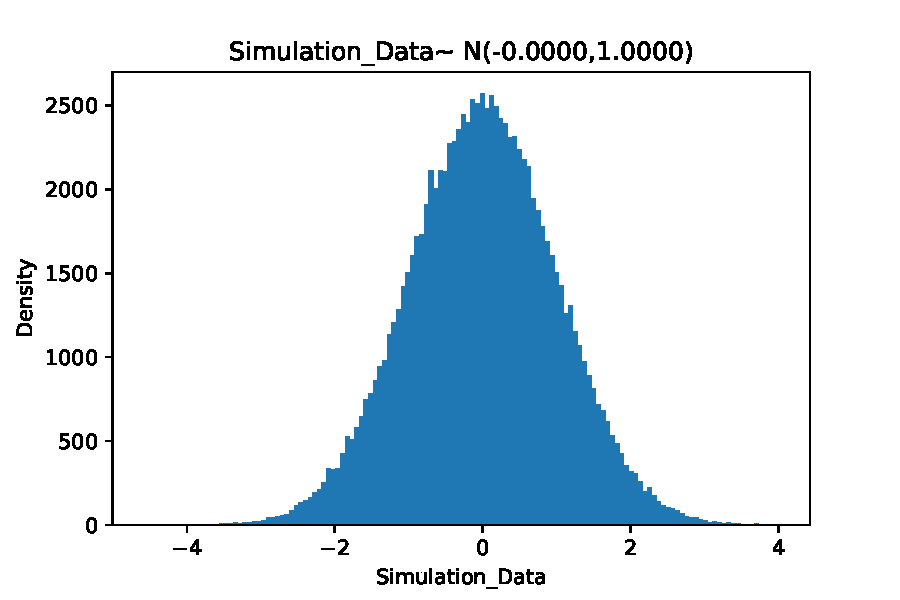
\includegraphics[width=1\textwidth]{Simulation/Bitwidths/Distribution.pdf}
        % \end{minipage}
    % }
    % \subfloat[Loss with different bit widths]{
        % \label{fig:loss}
        % \begin{minipage}[t]{0.48\textwidth}
        %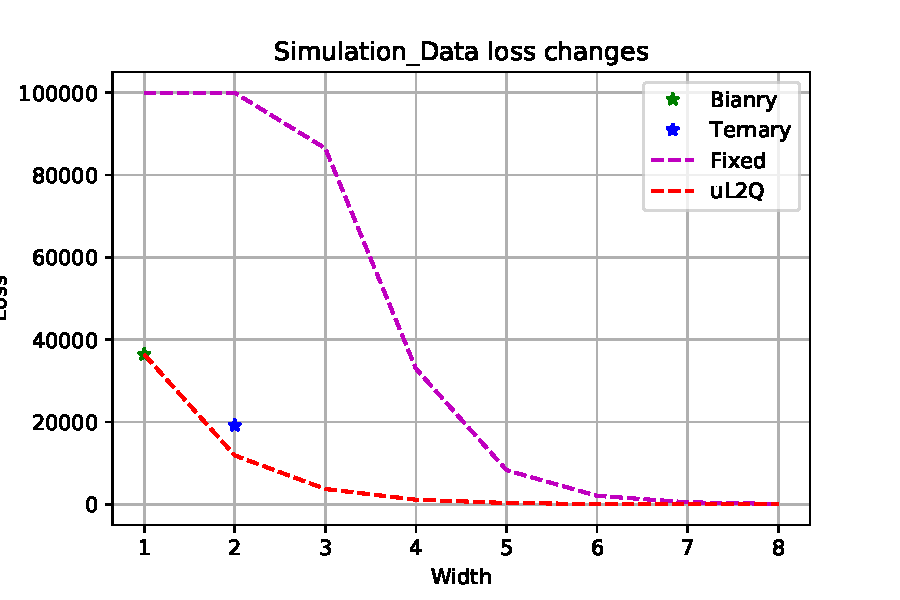
\includegraphics[width=0.48\textwidth]{Simulation/Bitwidths/LossWithWidth.pdf}
        % \end{minipage}
    % }
    %\caption{Loss with different bitwidth.}
    %For the same data distribution, as shown in \figref{fig:dist}, the loss comparison of different quantization algorithms over different bit widths. From \figref{fig:loss}, Our quantization algorithm has the lowest loss in all bit widths.}
    %\label{fig:Loss_with_bits}
%\end{figure}

As shown in~\ref{fig:Loss_with_bits},
our quantification method maintains the lowest data loss over all bit widths. 
For binary quantization, which the quantized data occupied only 1 bit, we maintain the same data loss as~\cite{zhou2016dorefa}. It is worth noting that the loss of our method does not change with the mean value of the original data, 
but binary quantization in~\cite{zhou2016dorefa} could only provide a minimum data loss when the mean value is zero according to our experimental results.

The ternary quantizatio, the quantized data occupies 2 bits, the data loss of $\mu$L2Q at 2 bit is lower than the state-of-the-art results from~\cite{TWNs}. 
Ternary uses 2-bit resource to represent three values \{-1, 0, 1\}. Meanwhile, $\mu$L2Q fully use 2 bits with four values \{-1, 0, 1, 2\}. Therefore, the data loss of $\mu$L2Q is lower.

The loss of $\mu$L2Q is always lower than the fixed point quantization. The reason is that fixed point quantitation does not consider the normal distributed data characteristic. $\mu$L2Q take the data distribution into consideration and provides a more balanced quantization. 

%Fixed-point quantization can be performed on different quantization bit widths, but its high loss at low bit widths and its low utilization of bit width make it difficult to achieve better trade-offs between efficiency and loss.

% \begin{figure*}[!ht]
%     \flushleft
%     \begin{minipage}[t]{1\textwidth}
%             \flushleft
%             \begin{overpic}[width=0.24\textwidth]{Simulation/Bitwidths/BinaryDistribution.pdf}
%                 \put(-10,15){\rotatebox{90}{Binary}}
%                 \put(93,15){\rotatebox{90}{Ternary}}
%                 \put(-10,-50){\rotatebox{90}{Fixed}}
%                 \put(-10,-115){\rotatebox{90}{Our}}
%                 \put(40,70){1bit}
%                 \put(145,70){2bit}
%                 \put(250,70){4bit}
%                 \put(355,70){8bit}
%             \end{overpic}
%             %\includegraphics[width=0.24\textwidth]{fig/SingleFmeasure/bark_f1_single.pdf}
%             %\includegraphics[width=0.24\textwidth]{fig/Bitwidths/binary-results_1bit.pdf}
%             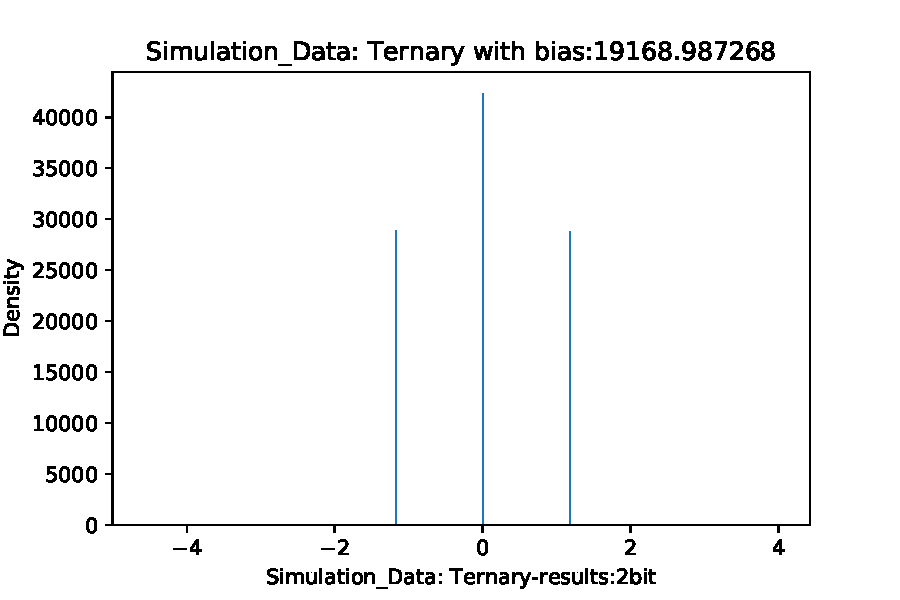
\includegraphics[width=0.24\textwidth]{Simulation/Bitwidths/TernaryDistribution.pdf}\\
%             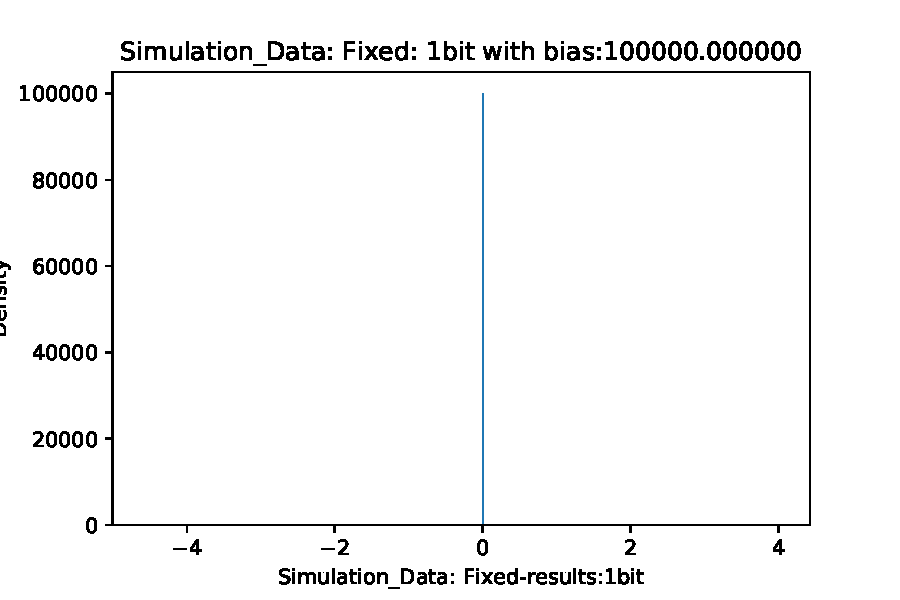
\includegraphics[width=0.24\textwidth]{Simulation/Bitwidths/FixedDistribution_1bit.pdf}
%             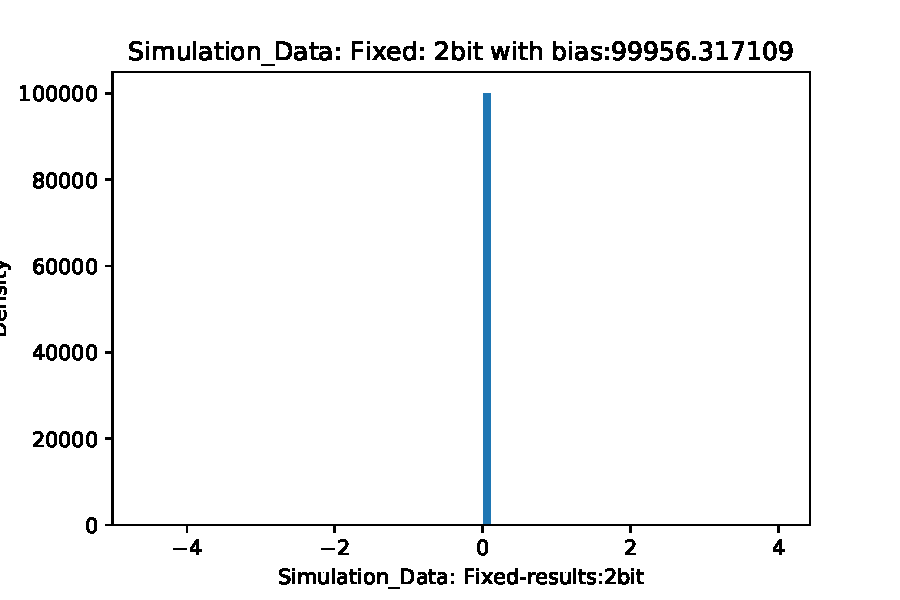
\includegraphics[width=0.24\textwidth]{Simulation/Bitwidths/FixedDistribution_2bit.pdf}
%             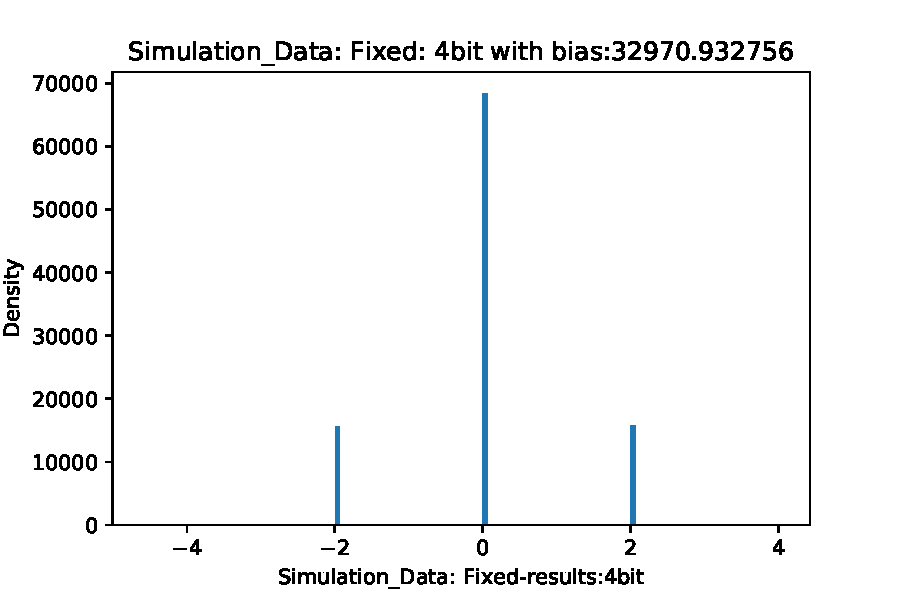
\includegraphics[width=0.24\textwidth]{Simulation/Bitwidths/FixedDistribution_4bit.pdf}
%             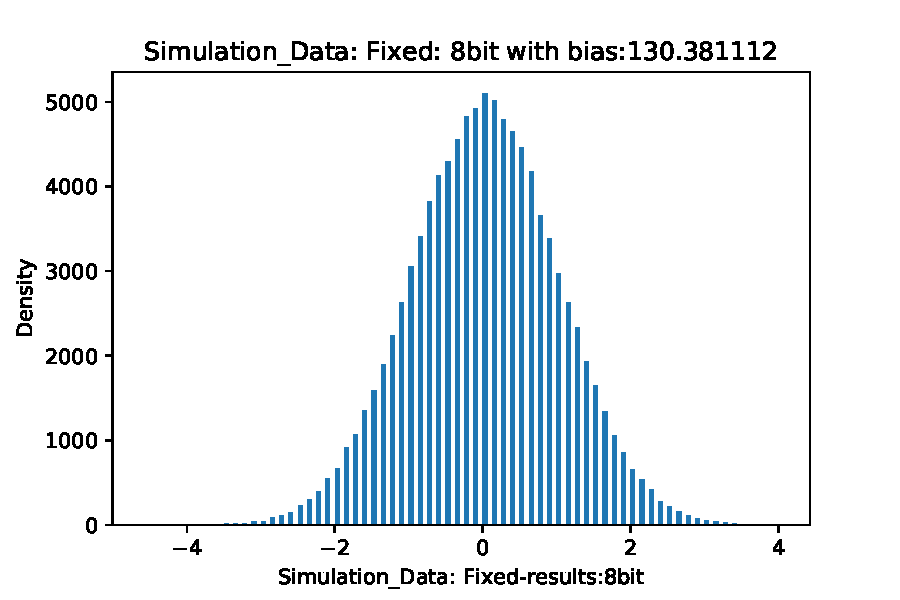
\includegraphics[width=0.24\textwidth]{Simulation/Bitwidths/FixedDistribution_8bit.pdf}\\
%             \includegraphics[width=0.24\textwidth]{Simulation/Bitwidths/$\mu$L2QDistribution_1bit.pdf}
%             \includegraphics[width=0.24\textwidth]{Simulation/Bitwidths/$\mu$L2QDistribution_2bit.pdf}
%             \includegraphics[width=0.24\textwidth]{Simulation/Bitwidths/$\mu$L2QDistribution_4bit.pdf}
%             \includegraphics[width=0.24\textwidth]{Simulation/Bitwidths/$\mu$L2QDistribution_8bit.pdf}
%             %\fbox{\rule[-. 5cm]{0cm}{4cm} \rule[-. 5cm]{4cm}{0cm}}
%     \end{minipage}
%     \caption{Quantized data distribution, original data distribution is shown in \figref{Data_distribution}. Compared with other quantization algorithms, our algorithm makes full use of the expression ability within the set bit width to quantize the original data to the maximum amount of information that can be carried by the set bit width.}
%     \label{fig:quantization_distribution}
% \end{figure*}

\subsubsection{Loss with different means and standard deviations}
%The actual network weights are often not standard normal distributed, and it is necessary to test the performance of the quantization algorithms on different normal distributions.
%Different quantization methods should be stable and robust on different normal distributions. We generate normal distribution data with different mean and standard deviations to test the performance of different quantization methods.
%\textbf{Results: }
As shown in \figref{fig:loss_with_distribution}, Our method is the most stable one among all the evaluated methods with the different means and standard deviations.
The loss of binary and ternary quantization increase as the mean shifts away from the origin, as is shown in~\figref{loss_with_means}.
%The fixed-point quantization does not support 1 bit due to the sign value but we still put the value there to ease comparison of the following values.
%is stable in 1 bit since fixed-point quantization can only be quantized to 0 when the bit width is 1 bit, that is, the sign bit. 
%\textcolor{red}{Remove the 1 bit for fixed, it does not support 1 bit.}
Fixed-point quantization fluctuates greatly at 2bit width, while it is stable at 4-bit and 8-bit since the bit width is sufficient for data representation. 
The data loss of $\mu$L2Q does not change with the mean value. What is more, the data loss of $\mu$L2Q at 1 bit can even achieve the same as fixed-point quantization with 4 bits data representation. 
%When the mean value is greater than 1, our method shows lower loss than any other methods.
Our method is also shows the most stability among all the other quantization methods with different standard deviations by taking advantage of taking the data distribution into consideration, as shown in \figref{loss_with_sds}. 
% As the standard deviation increases, the difference of data is prominent, and the loss of all quantization methods increases. The fixed-point quantified fluctuation is the greatest, and our method coincides with binary quantization at 1 bit width. Our method is the most stable, and the results at 2bit width has better than binary, ternary quantization, and fixed-point quantization's results at 4bit width.

%can achieve the lowest loss is that we fully consider the three factors: 1) Based on the standard normal distribution, we theoretically fully analyze the optimal choice of the quantized locations, which is the essential reason for our algorithm achieving the lowest loss; 2) We normalize all the data to the standard normal distribution and then quantify it, which not only ensures the premise of our theoretical analysis above, but also ensures that our method is insensitive to mean and keep stable for standard deviation change, which guarantees the robustness of our method; 3) We make full use of the bit-width resources, without wasting any representation bits. Our method can make full use of $2^k$ representation values for $k$-bit width resources. For example, as shown in \figref{fig:quantization_distribution}, on 1bit, our method quantizes to 2 values; on 2bit quantizes to 4 values, and the values are 16 and 256 on 4bit and 8bit respectively. In contrast, ternary quantization only uses 3 values of the 4 values, and the fixed-point quantization method has also no relevant guarantee.



\subsection{$\mu$L2Q for DNN training}
%数据集的选择
\subsubsection{Experimental settings}
% \textbf{Selection of datasets.}
Three well-known data sets are chosed for our experiments, which are Mnist \citep{mnist}, Cifar10 \citep{cifar10} and ImageNet \citep{deng2009imagenet}. 
% The size of the images in the three data sets is incremental, Mnist is the smallest, Cifar10 is larger, and ImageNet is the largest. 
% These three data sets are often used to evaluate the effectiveness of the compression method such as in \citep{TWNs,gysel2016hardware,Ternaryconnect}.
%基于数据集的网络模型选择
% \textbf{Selection of DNN models.}
Based on the above datasets, we select some widely used neural network models for our evaluations, including Lenet-5 \citep{lecun1998gradient} for Mnist, Cifarnet \citep{krizhevsky2009learning} and VGG7-64 \citep{simonyan2014vgg}\footnote{Network architecture is $3\times32\times32 (input)-C(3,64)-BN-C(3,64)-BN-MP2-C(3,128)-BN-C(3,128)-BN-MP2-C(3,256)-BN-C(3,256)-BN-F(1024)-BN-F(10)-Softmax$. C(K,O) denotes a convolution with kernel size $K\times K$ and $O$ outputs, MP2 stands for $2\times2$ max pooling, F(O) means the fully-connected layer with $O$ outputs, and BN represents batch normalization. 
} 
for Cifar10 and Resnet-18 \citep{he2016deep} for ImageNet. The effectiveness of our proposed method is evaluated with the illustration of it into Caffe training flow. 
% The final testing accuracy is the comparison metric. 
The network size in terms of parameter number and training settings for different models are shown in \tabref{tab:networktrainingmodel}.
\begin{table}[]
\caption{Model size and training parameter settings.}
\label{tab:networktrainingmodel}
\begin{tabular}{c|c|c|c|c}
\hline
Dataset                   & Mnist  & \multicolumn{2}{c|}{Cifar10} & Imagenet  \\\hline
Model                     & Lenet5 & Cifarnet     & VGG7-64      & Resnet-18 \\\hline
Parameter number(M)             & 0.43 & 0.279      & 5.35       & 11.69   \\\hline
Weight decay              & 0.0004 & 0.0001       & 0.0004       & 0.0001    \\
Batch size                & 100     & 100          & 100          & 64*4      \\
Initial learning rate     & 0.01   & 0.0001       & 0.01         &   0.1        \\
Learning rate decay & 0.1  & 0.1    & 0.2     &         0.1  \\
Learning rate decay epoch & 32,48  & 120,130      & 16,32,36     &     30,40,50      \\
Momentum                  & 0.9    & 0.9          & 0.9          & 0.9    \\\hline  
\end{tabular}
\end{table}

\textbf{Existing quantization methods for comparing.}
Many existing quantization methods including the state-of-the-art ones are chosen for comparison.
These methods can be divided into three categories. 
Firstly, binary quantization methods, including RebNet \citep{ghasemzadeh2018rebnet}, BNN \citep{BitwiseNN}, BPWNs \citep{TWNs}, BWN \citep{rastegari2016xnor}, XNOR-NET \citep{rastegari2016xnor} and BC \citep{Binaryconnect}. 
Secondly, ternary quantization methods are chosen, including TNN \citep{alemdar2017ternary}, TN \citep{TrueNorth1}, TWNs \citep{TWNs}, STC \citep{jin2018sparse} and TC \citep{Ternaryconnect}. 
Finally, some certain bitwidths of fixed-point quantization results from hardware~\cite{gysel2016hardware} are also chosen to compare with the results of our $\mu$L2Q. 
All the comparison targets are concluded in \tabref{tab:comparisionmethods}.
\begin{table}[]
    \centering
    \caption{Comparison targets.}
    \label{tab:comparisionmethods}
    \begin{tabular}{c|c}
        \hline
        Category & Methods \\\hline
        \multirow{2}{*}{Binary} & RebNet \citep{ghasemzadeh2018rebnet}, BNN \citep{BitwiseNN}, BPWNs \citep{TWNs}, \\
                & BWN \citep{rastegari2016xnor}, XNOR-NET \citep{rastegari2016xnor}, BC \citep{Binaryconnect}\\\hline
        Ternary & TNN \citep{alemdar2017ternary}, TN \citep{TrueNorth1}, TWNs \citep{TWNs}, STC \citep{jin2018sparse} and TC \citep{Ternaryconnect} \\\hline
        Fixed-point& hardware \cite{gysel2016hardware}\\\hline
        \textbf{Ours}&$\mu$L2Q\\\hline
    \end{tabular}
\end{table}

\textbf{Training configuration and result settings of $\mu$L2Q.} 
$\mu$L2Q can achieve data quantization at any bit width. 
For simplicity of description, we use $\mu$L2Q-x to denote $\mu$L2Q quantized data at x-bit width.
$\mu$L2Q-x compresses the network's weights, including weights of convolution and fully-connected layer to x-bit width. 
However, considering that the last fully-connected layer has a greater impact on the accuracy of the model, we only quantize the last fully-connected layer to 8/16 bits or maintain it as floating point.

\begin{figure*}[htp]
\centering
\subfloat[Lenet5]{
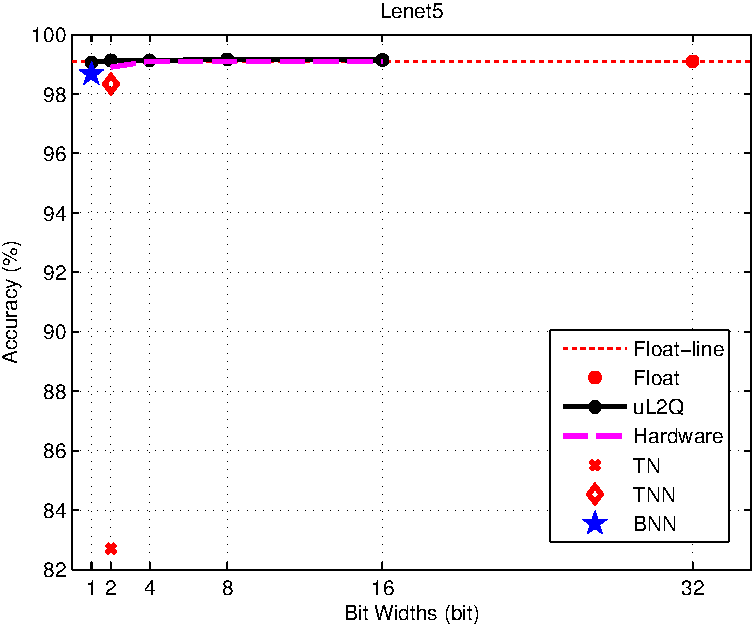
\includegraphics[width=0.31\textwidth]{fig/Lenet5_accuracy_bits.pdf}
\label{fig:lenet5acc}
}
\subfloat[Cifarnet]{
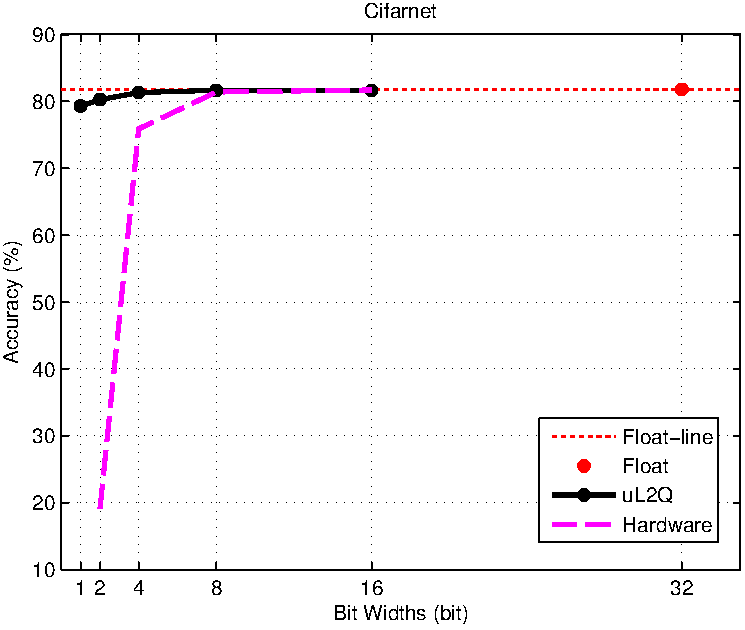
\includegraphics[width=0.31\textwidth]{fig/Cifarnet_accuracy_bits.pdf}
\label{fig:cifarnetacc}
}
\subfloat[VGG7-64]{
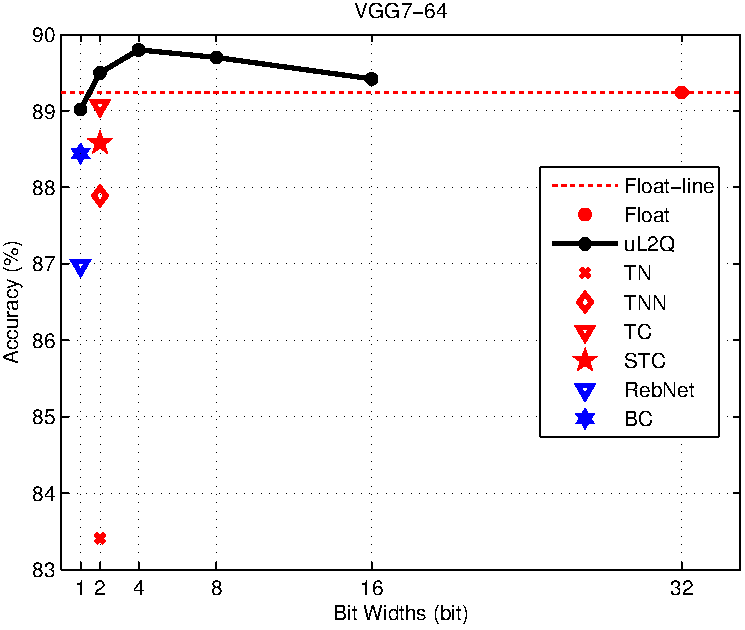
\includegraphics[width=0.31\textwidth]{fig/VGG7-64_accuracy_bits.pdf}
\label{fig:vgg764acc}
}\\
\subfloat[ResNet-18 Top1]{
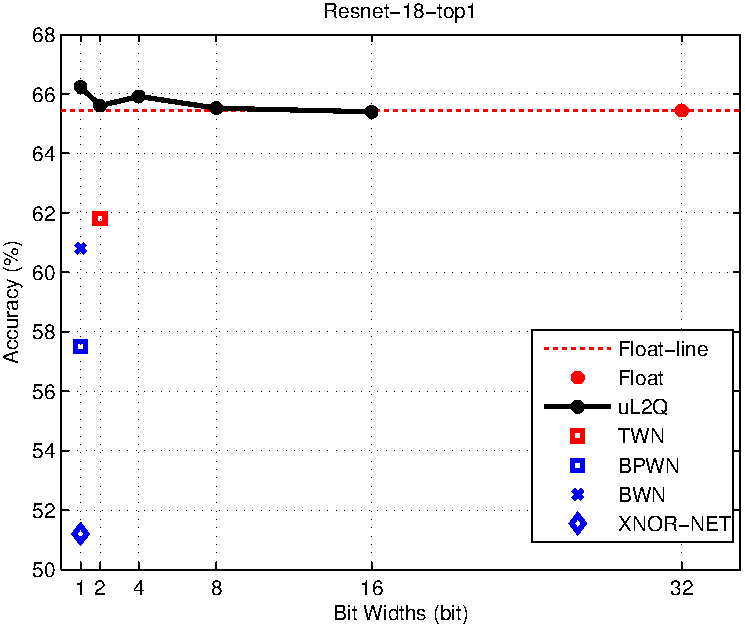
\includegraphics[width=0.31\textwidth]{fig/Resnet-18-top1_accuracy_bits.pdf}
\label{fig:resnet181acc}
}
\subfloat[ResNet-18 Top1]{
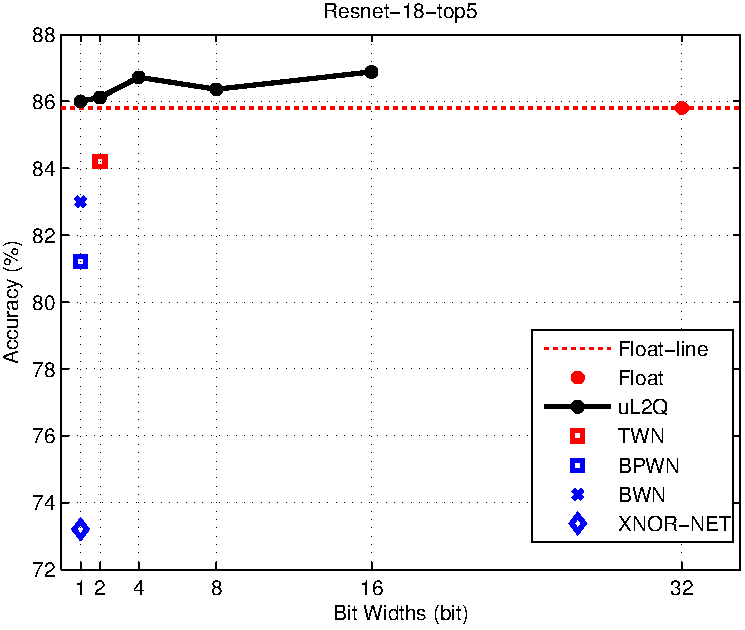
\includegraphics[width=0.31\textwidth]{fig/Resnet-18-top5_accuracy_bits.pdf}
\label{fig:resnet185acc}
}

\caption{The output accuracy of the model under different weight bit widths. The x-axis is the bit width of the model weights, and the y-axis is the output accuracy of the model. Float is the output of a full-precision weight model with 32-bit floating-point numbers, and Float-line is a horizontal line equal to the Float accuracy used for comparison.}
\label{fig:accuracy_at_bits}
\end{figure*}

\textbf{Result Analysis.} All of our comparison results are shown in Table 5. $\mu$L2Q-x and Hardware-x represent the results at x-bit width. \figref{fig:accuracy_at_bits} shows the outputs of the models at different bit widths. For objective comparison, we directly quoted the experimental results in the literature.

\textcolor{blue}{$\mu$L2Q vs Binary.} On the chosen datasets and network models, results of $\mu$L2Q at 1 bit perform better than the ones of binary methods. 
Network weights generally is not a data with standard normal distribution, but with some mean shift and standard deviation scaling. 
$\mu$L2Q is invariant about the mean shift, and is stable about the standard deviation scaling. But the binary method is unstable about these transformations, and this lead to the accuracy degradation of binary methods.

\textcolor{blue}{$\mu$L2Q vs Ternary.} At the 2 bit width, $\mu$L2Q perform better than the ternary methods, even exceed the results of float weights on some models (exceed the Float-line in \figref{fig:accuracy_at_bits}). There are two main reasons for the accuracy degradation of ternary methods. One, like the binary methods' defect, is the instability about the transformation of mean shift and the standard deviation scaling. The second reason is the waste of bit width resources. The value of ternary weights only hold three values, and its storage bit width is at least 2 bits. Meanwhile, 2 bit widths can represent up to 4 values. The expression of 4 values is much larger than 3 values, and its storage requirements are the same as the ternary. $\mu$L2Q uses four values at the 2 bit width, so its model accuracy are better than the results of the ternary methods.

\textcolor{blue}{$\mu$L2Q vs Fixed-point.} The representative method of fixed-point quantization is Hardware \citep{gysel2016hardware}. For fair comparison, we only reference the results with quantized convolution weigths in Hardware, that is, the full connection weigths are full precision. It is worth noting that Hardware had no result at 1 bit width, and its lowest bit width is 2.
Since the Mnist data set is small, Hardware and $\mu$L2Q perform similarly on Lenet5. 
On cifarnet, when the bit width is enough, the results of Hardware and $\mu$L2Q are very similar, and the accuracy degradation of both is small.
However, at low bit widths ($<4$bit), Hardware's results are poor (only 19.10\% at 2bit and 75.90\% at 4bit), and it is consistent with our prior analysis (\secref{sec:fixed-point}), that is, fixed-point quantization is poor at low bit widths. In contrast, when $\mu$L2Q at low bit widths, the results are stable. Even the result of 1bit has exceeded the result of hardware in 4bit ($\mu$L2Q-1:79.28\% $>$ Hardware-4:75.90\%).

\textcolor{blue}{$\mu$L2Q vs bitwidths} Analysis of $\mu$L2Q's results at different bit widths.
On the small network models, such as Lenet5 and Cifarnet, the accuracy of $\mu$L2Q is increasing by bit width, which is reasonable. Since the small models have less parameters, it have less redundancy,  and is easy to under-fitting. More bit widths can have more complex expressions to prevent under-fitting, so the accuracy is increasing with bit-width.
On large models, such as VGG7-64, and Resnet18, the accuracy of $\mu$L2Q is not consistent with the increase of bit width, but occur some fluctuations. $\mu$L2Q-4 outputs the highest accuracy on VGG7-64,  higher than the full precision results. $\mu$L2Q-1 has the best results on TOP1 of ResNet-18. Meanwhile, $\mu$L2Q-16 has the best results on TOP5 of ResNet-18. Large models have too many parameters, they are highly redundant and easy to over-fitting. The weights with low bit widths can reduce model complexity and prevent over-fitting,  and improve the generalization ability (test accuracy) of the model. However, too low bit widths of weights can also lead to under-fitting. Therefore, the best results of the model will only appear on the appropriate bit width.
Another interesting phenomenon is that on ResNet-18, the output accuracy of TOP1 is decreasing, while the output accuracy of TOP5 is increasing. This denotes that the redundancy of the model depends not only on the parameter number of model and the size of the data set, but also on the output of model. When the previous two conditions are given, the more complex of model's output is, the less model's redundancy is, and it is not easy to over-fitting, but easy to under-fitting. When the output is simple, it is easy to over-fitting.

%总结一下
\textcolor{blue}{$\mu$L2Q vs Float.}
$\mu$L2Q perform well on different models. Its results even are better than the ones of full precision model except Cifarnet, and it is reasonable and interpretable. These models have a certain degree of over-fitting, and low precision (bit width) of weights can reduce the complexity of the model, prevent over-fitting, and improve the generalization ability (test accuracy) of the model. Cifarnet is a special case. The parameters of the Cifarnet model are small (the parameter quantity is only 65.88\% of Lenet5), which is easy to under-fitting and needs to increase the complexity of the model to improve the performance of it. However, $\mu$L2Q is used to reduce the precision of weights and does not solve the problem of under-fitting, so it is slightly lower than the full-precision result on Cifarnet. 

%The final trained DNN performance in terms of classification accuracy is shown in Table~\ref{tab:accuracy_comp}.
%在两个模型上比全精度高
%$\mu$L2Q exceeds the output of the full precision model on both the Lenet5 and VGG7-like models. This is mainly because the two models have much parameters and great redundancy considering the data set. Therefore, quantization can remove redundancy and prevent over-fitting, which improves a certain precision.
%在Cifarnet上
%Cifarnet has few parameters, even fewer parameters than Lenet5, and its redundancy is small. The general quantization method has a great influence on the output of this model. For example, the hardware-2 (2bit) output accuracy is only 19.10\%. Meanwhile, the accuracy of $\mu$L2Q-2 (2bit) is as high as 80.26\%. Therefore, $\mu$L2Q has great advantages in low bit width quantization, and $\mu$L2Q is also ideal in high bit width.

% Please add the following required packages to your document preamble:
% \usepackage{multirow}
\begin{table}[]
\center
\caption{Accuracy(\%) comparison.}
%C is the convolutional bit width, F is the full-connection bit width, LF is the last full-connection layer bit width, and G is the gradient bit width.}
\label{tab:accuracy_comp}
\begin{tabular}{l|c|c|c|c}
\hline
Datasets    & Mnist  &\multicolumn{2}{c|}{Cifar10}   & ImageNet \\ \hline \hline
Model       & Lenet5 & Cifarnet & VGG7-like & ResNet-18(Top1/5)\\ \hline
Float       & 99.10  & 81.82    & 89.24  &65.44/85.80 \\\hline
ReBNet(M=3)\citep{ghasemzadeh2018rebnet} & -  &  -        & 86.98  &- \\
BitwiseNN\citep{BitwiseNN} &	98.67 &		- &-\\
BPWNs\citep{TWNs}  & -  &  -        & -  &57.50/81.20 \\
BWN\citep{rastegari2016xnor}  & -  &  -        & -  &60.80/83.00 \\
XNOR-NET\citep{rastegari2016xnor}  & -  &  -        & -  &51.20/73.20 \\
BC\citep{Binaryconnect}		&-&-&	88.44 &-\\\hline
TNN\citep{alemdar2017ternary}         & 98.33  &  -        & 87.89  &- \\
TrueNorth\citep{TrueNorth1} &	82.70 &		& 83.41 &- \\
TWNs\citep{TWNs}   & -  &  -        & -  &61.80/84.20 \\
STC\citep{jin2018sparse}&-&-&88.58&-\\
TC\citep{Ternaryconnect}		&-&-&	89.07&-\\\hline
Hardware-2\citep{gysel2016hardware} &	98.90 &	19.10 &-&-\\
Hardware-4\citep{gysel2016hardware} &	99.10 &	75.90 &-&-\\
Hardware-8\citep{gysel2016hardware} &	99.10 &	81.40 &-&-\\
Hardware-16\citep{gysel2016hardware} &	99.10 &	81.70 &-&-\\\hline
\textbf{$\mu$L2Q-1}       & 99.06  & 79.28    & 89.02  &66.24/86.00 \\
\textbf{$\mu$L2Q-2}       & 99.12  & 80.26    & 89.50 &65.60/86.12\\
\textbf{$\mu$L2Q-4}       & 99.12  & 81.32    & 89.80 &65.92/86.72 \\
\textbf{$\mu$L2Q-8}       & 99.16  & 81.66    & 89.70 &65.52/86.36 \\
\textbf{$\mu$L2Q-16}      & 99.14  &  81.64   & 89.42  &65.40/86.88 \\
\hline
\end{tabular}
\end{table}

%\textcolor{red}{Please add the analysis of the results in the table here. Only finish this part after your results in the table are good enough!!!}

\section{Conclusion}\label{sec:con}
%In this paper, we analyze some problems of currently quantization methods, such as the strong subjectivity of researchers, based on experience guidance rather than theory and so on. Based on the existing problems, we propose ULQ, which is based on the assumption that the weights satisfy the normal distribution. We fully analyze the best solution that ULQ can theoretically achieve. Theoretical analysis shows that the optimal solution of ULQ has no straightforward solutions. But we novelly solve this problem by normalizing weights to a standard normal distribution. By limiting the conditions, we can solve this problem by enumerating all the data. Finally, in our experimental part, we verify the correctness of our theoretical analysis by simulating a complete normal distribution, and verify our assumption is reasonable through analysing the actual weights of the classical model, that is, most of the model weights satisfy the normal distribution.
In this paper, we realize that making assumptions about raw data is crucial. First, it limits the problem to a certain extent, rather than trying to solve all problems in one way. Second, it allows our method to be analyzed, and we can try to solve the problem using the tools in mathematical or machine learning,. This means that for differently distributed data, we should consider different methods to achieve lower data loss. 
In addition, we also find that the flexibility of quantization is the key to achieving precision and bit width trade-off. The fixed bit width based quantization method is difficult to apply to different DNN models, even if the weights of these models are all equal to the same distribution (such as the normal distribution).
%\emph{Future works: }Our future works will be the applying of ULQ to model training.
\section{Acknowledgement}
This work is partially supported by the National Natural Science Foundation (61872200, 11801284), the Natural Science Foundation of Tianjin (17JCQNJC00300), the Science and Technology Commission of Tianjin Binhai New Area (BHXQKJXM-PT-ZJSHJ-2017005) and the National Key Research and Development Program of China (2016YFC0400709).


\bibliographystyle{plain}
\bibliography{references}

%\appendix
%
We show the first 2 layer weights in \figref{fig:quantization_for_actualweights}, and all results can be found in our \emph{supplementary}.
As shown in \figref{fig:quantization_for_actualweights}, On the classic five models, our ULQ has the lowest loss. From the actual model, most of the actual weights satisfy the normal distribution, especially the batch-norm-based models, whose weights are normally distributed, which means that the premise we made is reasonable.

\begin{figure*}[!ht]
    \flushleft
    \begin{minipage}[t]{1\textwidth}
            \flushleft
            \begin{overpic}[width=0.24\textwidth]{ActualWeights/Lenet-5/conv1/Distribution.pdf}
                \put(-10,15){\rotatebox{90}{Lenet-5}}
                \put(-10,-50){\rotatebox{90}{Cifarnet}}
                \put(-10,-115){\rotatebox{90}{Resnet-18}}
                \put(40,70){conv1}
                \put(145,70){loss}
                \put(250,70){conv2}
                \put(355,70){loss}
            \end{overpic}
            %\includegraphics[width=0.24\textwidth]{fig/SingleFmeasure/bark_f1_single.pdf}
            %\includegraphics[width=0.24\textwidth]{fig/Bitwidths/binary-results_1bit.pdf}
            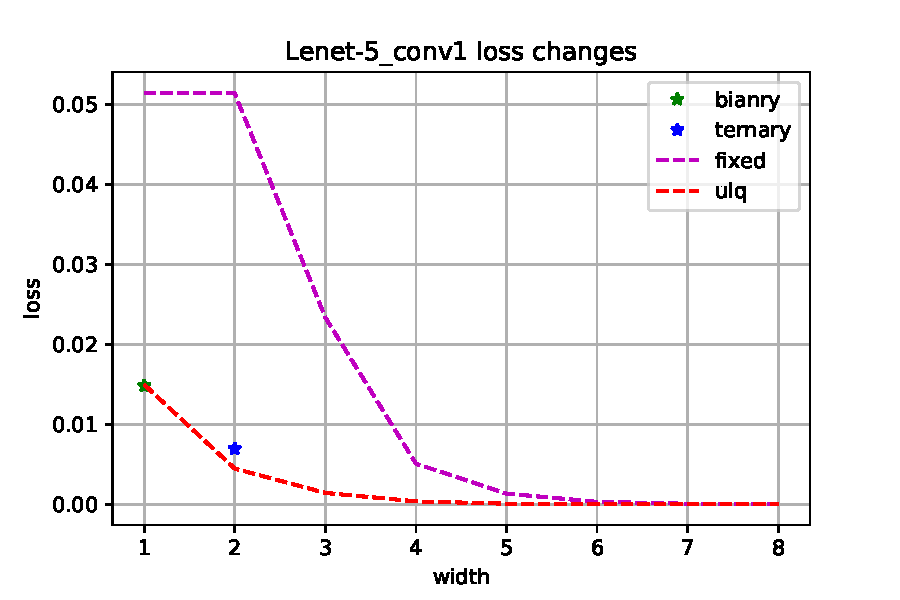
\includegraphics[width=0.24\textwidth]{ActualWeights/Lenet-5/conv1/LossWithWidth.pdf}
            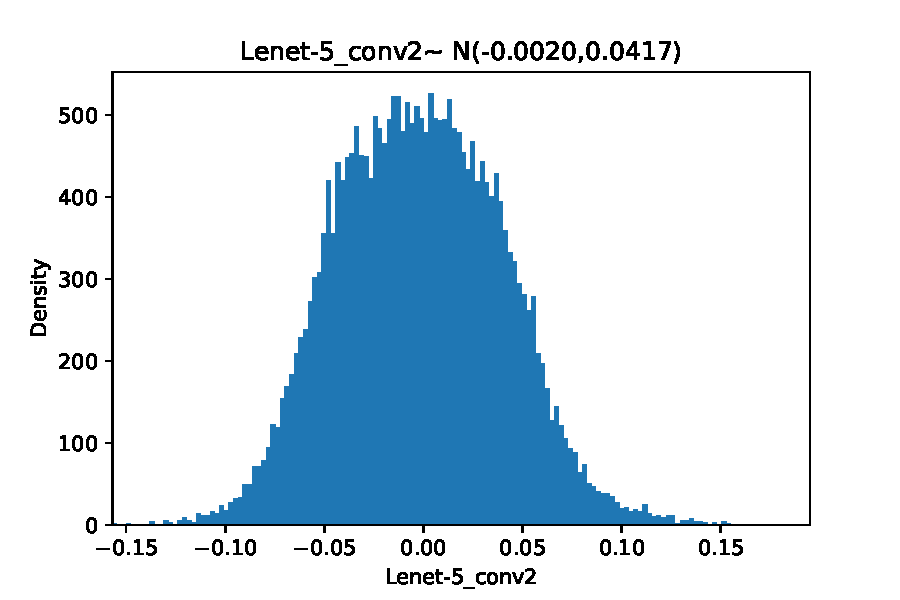
\includegraphics[width=0.24\textwidth]{ActualWeights/Lenet-5/conv2/Distribution.pdf}
            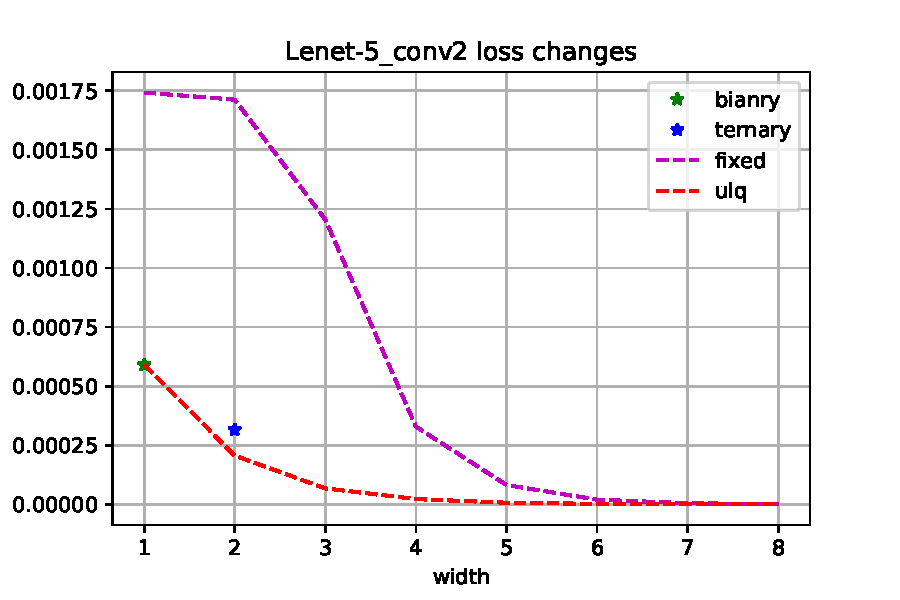
\includegraphics[width=0.24\textwidth]{ActualWeights/Lenet-5/conv2/LossWithWidth.pdf}\\
            
            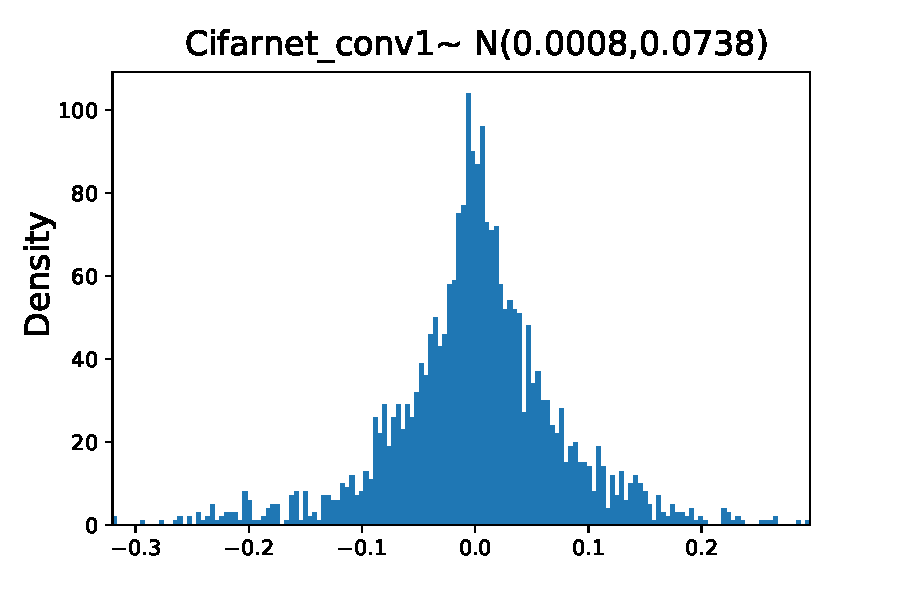
\includegraphics[width=0.24\textwidth]{ActualWeights/Cifarnet/conv1/Distribution.pdf}
            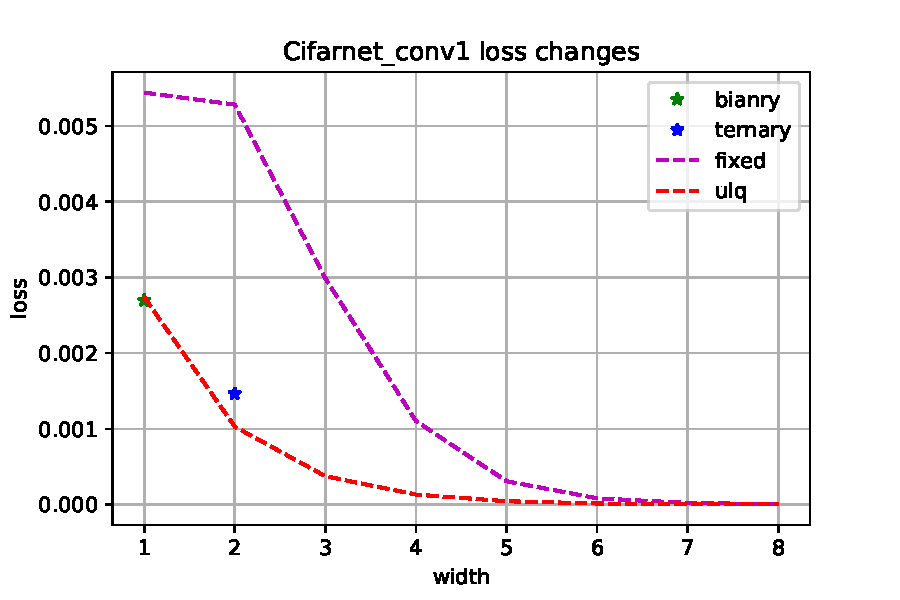
\includegraphics[width=0.24\textwidth]{ActualWeights/Cifarnet/conv1/LossWithWidth.pdf}
            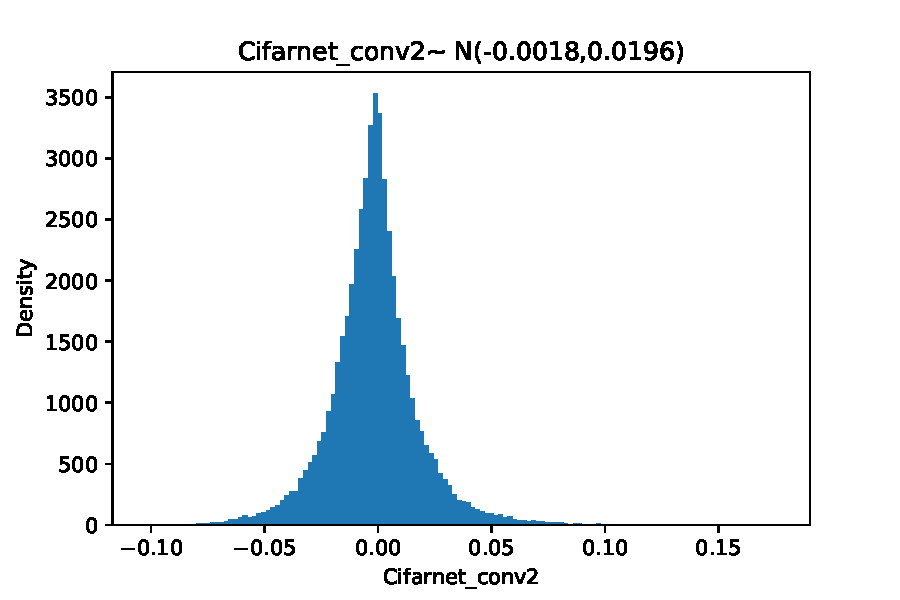
\includegraphics[width=0.24\textwidth]{ActualWeights/Cifarnet/conv2/Distribution.pdf}
            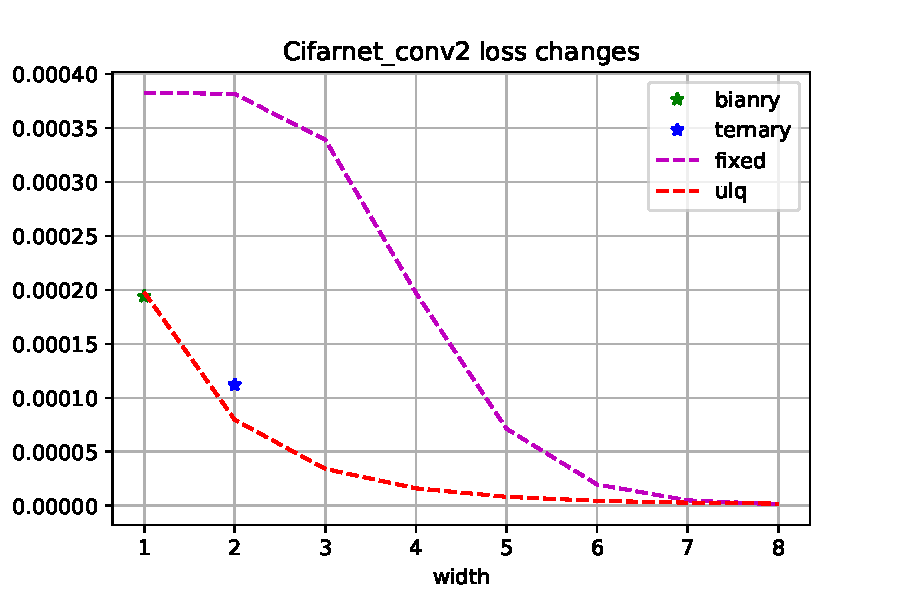
\includegraphics[width=0.24\textwidth]{ActualWeights/Cifarnet/conv2/LossWithWidth.pdf}\\
            
            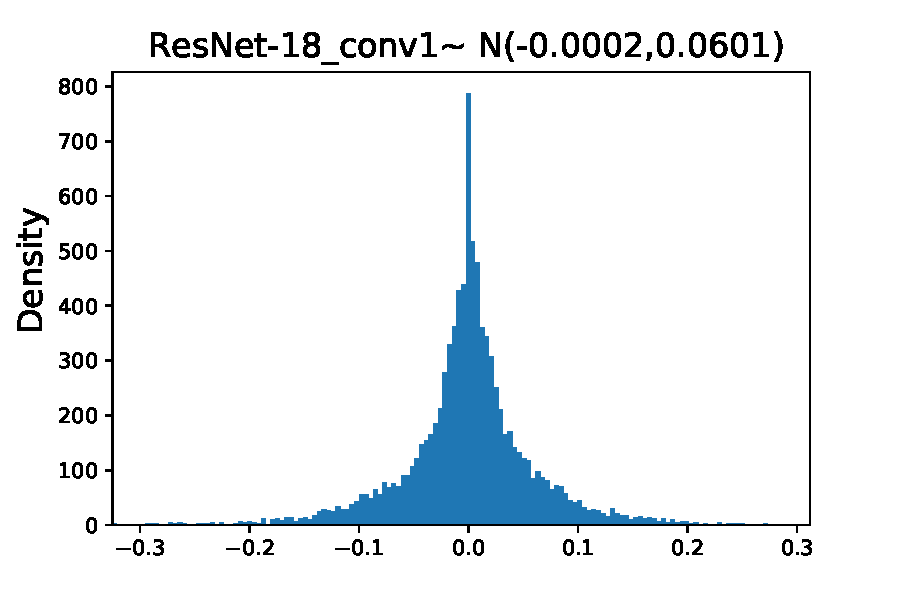
\includegraphics[width=0.24\textwidth]{ActualWeights/Resnet-18/conv1/Distribution.pdf}
            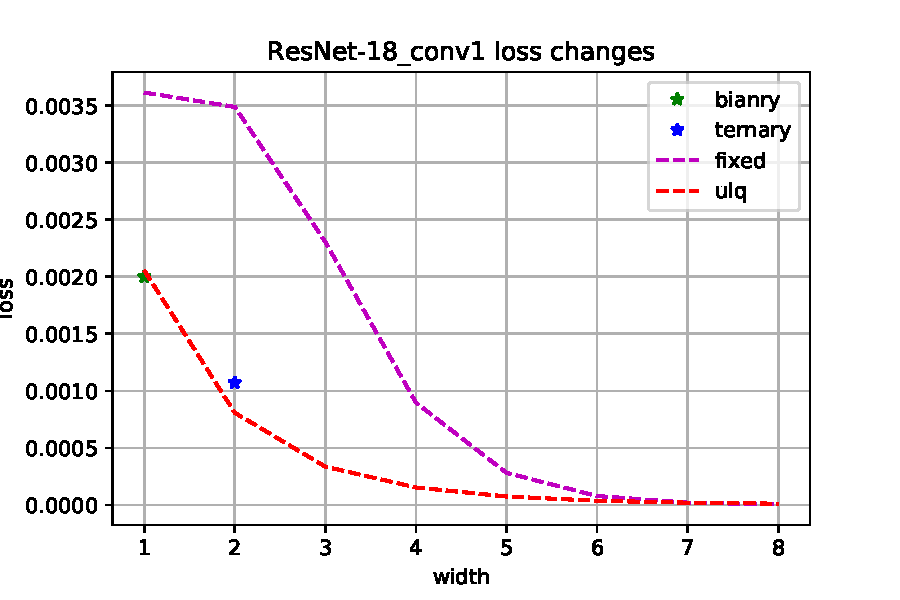
\includegraphics[width=0.24\textwidth]{ActualWeights/Resnet-18/conv1/LossWithWidth.pdf}
            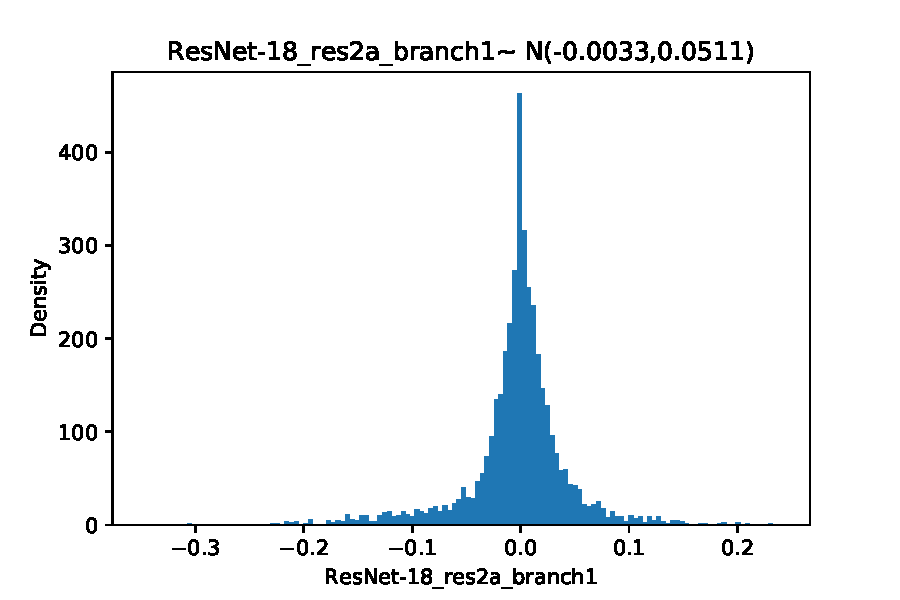
\includegraphics[width=0.24\textwidth]{ActualWeights/Resnet-18/branch1/Distribution.pdf}
            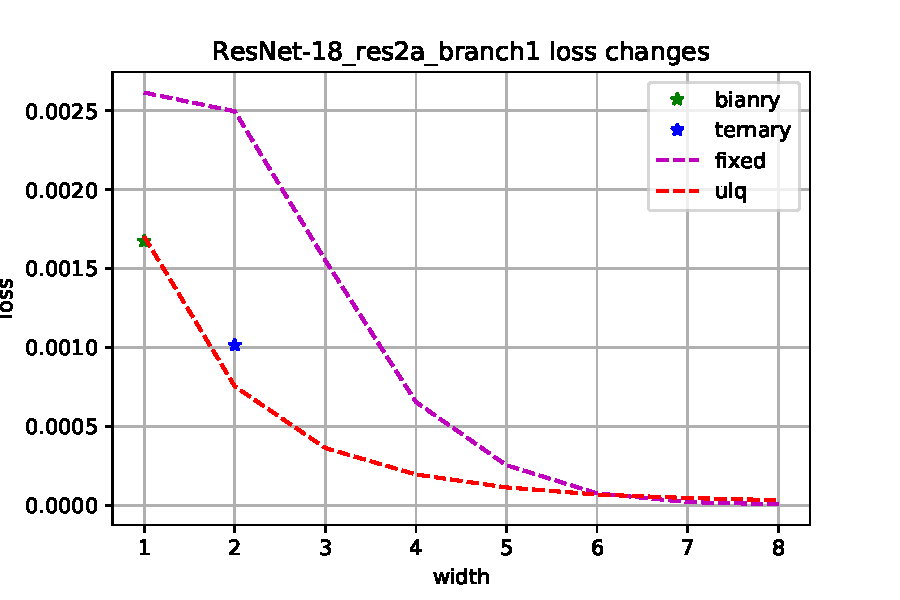
\includegraphics[width=0.24\textwidth]{ActualWeights/Resnet-18/branch1/LossWithWidth.pdf}
            %\fbox{\rule[-. 5cm]{0cm}{4cm} \rule[-. 5cm]{4cm}{0cm}}
    \end{minipage}
    \caption{Quantization comparision for the first 2 layers of models. All the weights satisfy the normal distribution and ULQ keeps the lowest loss in all results.}
    \label{fig:quantization_for_actualweights}
\end{figure*}

\end{document}
